%!TEX TS-program = xelatex
\documentclass[14pt, a4paper]{extarticle}\usepackage[]{graphicx}\usepackage[]{color}
%% maxwidth is the original width if it is less than linewidth
%% otherwise use linewidth (to make sure the graphics do not exceed the margin)
\makeatletter
\def\maxwidth{ %
  \ifdim\Gin@nat@width>\linewidth
    \linewidth
  \else
    \Gin@nat@width
  \fi
}
\makeatother

\definecolor{fgcolor}{rgb}{0.345, 0.345, 0.345}
\newcommand{\hlnum}[1]{\textcolor[rgb]{0.686,0.059,0.569}{#1}}%
\newcommand{\hlstr}[1]{\textcolor[rgb]{0.192,0.494,0.8}{#1}}%
\newcommand{\hlcom}[1]{\textcolor[rgb]{0.678,0.584,0.686}{\textit{#1}}}%
\newcommand{\hlopt}[1]{\textcolor[rgb]{0,0,0}{#1}}%
\newcommand{\hlstd}[1]{\textcolor[rgb]{0.345,0.345,0.345}{#1}}%
\newcommand{\hlkwa}[1]{\textcolor[rgb]{0.161,0.373,0.58}{\textbf{#1}}}%
\newcommand{\hlkwb}[1]{\textcolor[rgb]{0.69,0.353,0.396}{#1}}%
\newcommand{\hlkwc}[1]{\textcolor[rgb]{0.333,0.667,0.333}{#1}}%
\newcommand{\hlkwd}[1]{\textcolor[rgb]{0.737,0.353,0.396}{\textbf{#1}}}%
\let\hlipl\hlkwb

\usepackage{framed}
\makeatletter
\newenvironment{kframe}{%
 \def\at@end@of@kframe{}%
 \ifinner\ifhmode%
  \def\at@end@of@kframe{\end{minipage}}%
  \begin{minipage}{\columnwidth}%
 \fi\fi%
 \def\FrameCommand##1{\hskip\@totalleftmargin \hskip-\fboxsep
 \colorbox{shadecolor}{##1}\hskip-\fboxsep
     % There is no \\@totalrightmargin, so:
     \hskip-\linewidth \hskip-\@totalleftmargin \hskip\columnwidth}%
 \MakeFramed {\advance\hsize-\width
   \@totalleftmargin\z@ \linewidth\hsize
   \@setminipage}}%
 {\par\unskip\endMakeFramed%
 \at@end@of@kframe}
\makeatother

\definecolor{shadecolor}{rgb}{.97, .97, .97}
\definecolor{messagecolor}{rgb}{0, 0, 0}
\definecolor{warningcolor}{rgb}{1, 0, 1}
\definecolor{errorcolor}{rgb}{1, 0, 0}
\newenvironment{knitrout}{}{} % an empty environment to be redefined in TeX

\usepackage{alltt}
% Математика %
\usepackage{amsmath,amsfonts,amssymb,amsthm,mathtools}

% Шрифты 
\usepackage[british,russian]{babel} % выбор языка для документа
\usepackage[utf8]{inputenc} % задание utf8 кодировки исходного tex файла
\usepackage[X2,T2A]{fontenc}        % кодировка

\usepackage{fontspec}         % пакет для подгрузки шрифтов
\setmainfont{Arial}   % задаёт основной шрифт документа

\usepackage{unicode-math} 
\usepackage{tipa} % пакет для установки математического шрифта
%\setmathfont{Asana Math}      % шрифт для математики

\usepackage[paper=a4paper,top=10.5mm, bottom=10.5mm, left=10.5mm, right=10.5mm, includefoot]{geometry}
\usepackage[unicode,colorlinks=true,urlcolor=blue,hyperindex,breaklinks]{hyperref}
\setlength{\parindent}{0em}

\usepackage{booktabs} 
\usepackage{float}
\usepackage{graphics}
\usepackage{graphicx}
\usepackage{wrapfig} 
\usepackage{multicol}

\author{Семёнова Алёна}
\title{Эссе по временным рядам}
\date{20 апреля 2019 г.}
\IfFileExists{upquote.sty}{\usepackage{upquote}}{}
\begin{document}

\maketitle




\begin{center}
\section{Ряд 1. Погибшие в ДТП}
\subsection{Идентификация параметров и определение коэффициентов}
\end{center}

С сайта ЕМИСС выгрузила месячные данные по числу лиц, погибших в ДТП, в г. Москва с января $2010$ по апрель $2019$, $n = 112$. В исходном виде данные были оформлены в виде накопленного показателя, я преобразовала их в месячные данные, взяв соответсвующие разности. 
Посмотрим на графики данных:

\begin{figure}[H]
\begin{knitrout}
\definecolor{shadecolor}{rgb}{0.969, 0.969, 0.969}\color{fgcolor}

{\centering 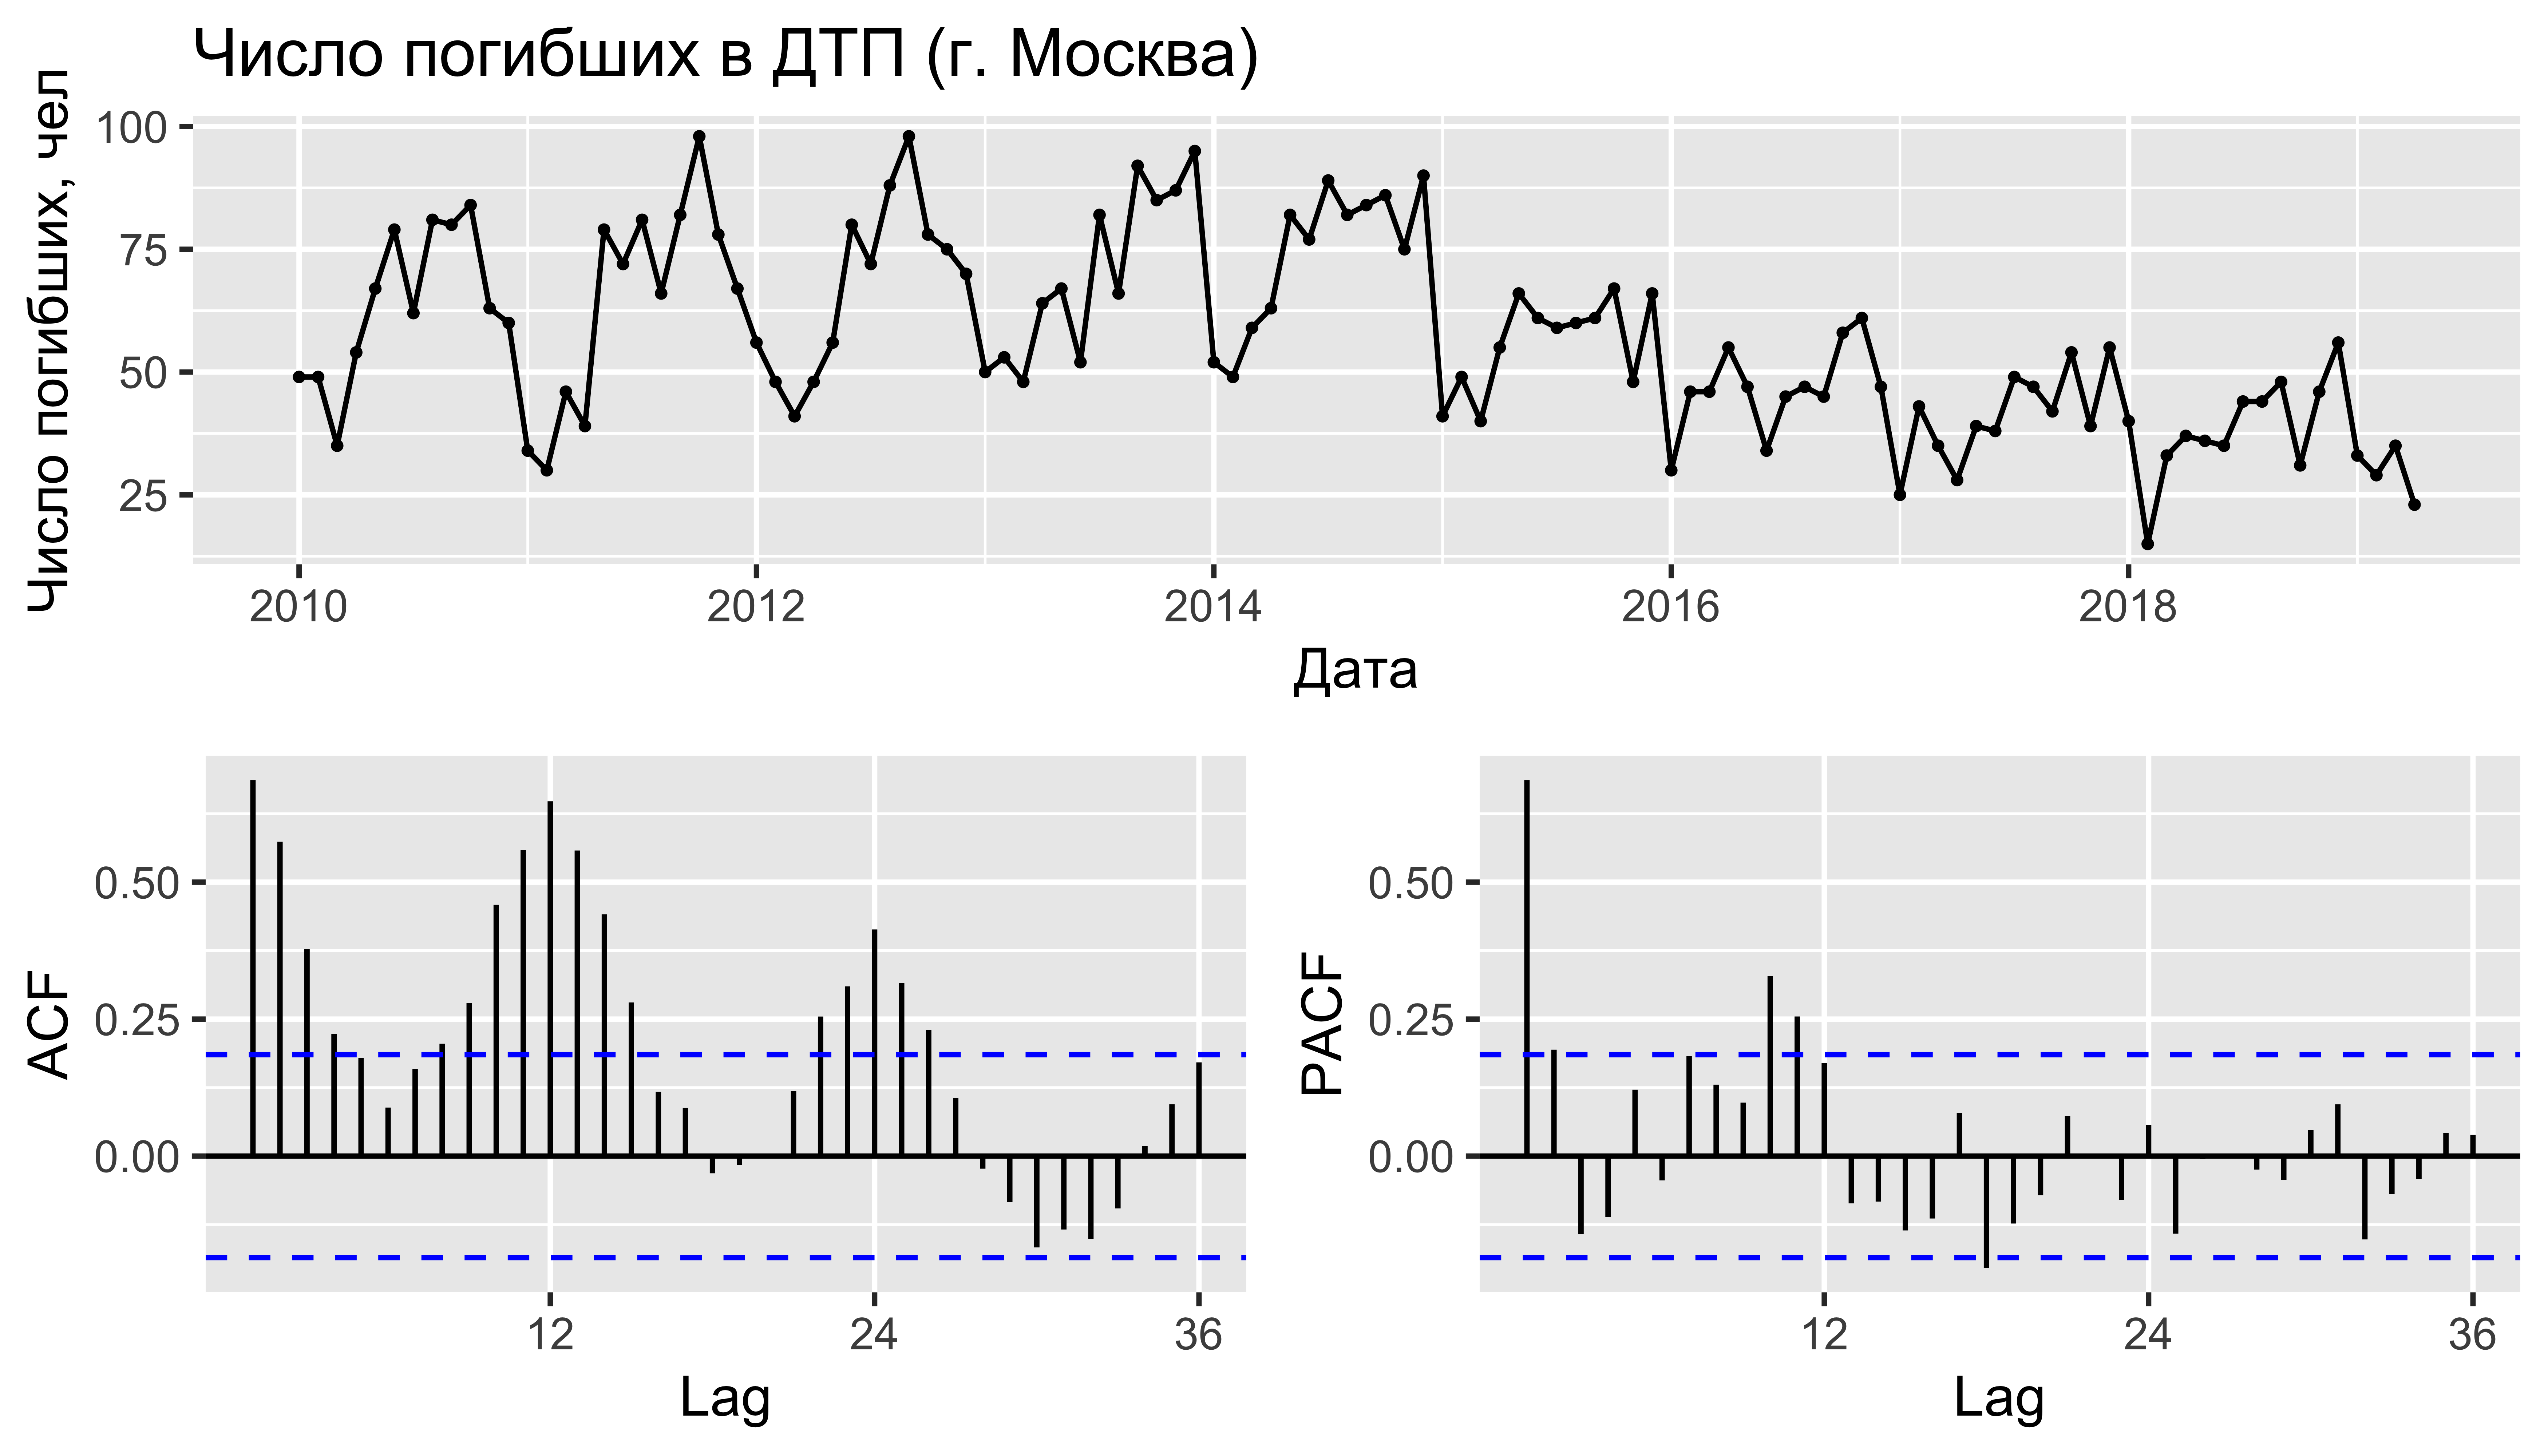
\includegraphics[width=\maxwidth]{figure/unnamed-chunk-1-1} 

}



\end{knitrout}
\end{figure}

Визуально на графике можно выявить:

\begin{enumerate}

\item Сезонность: в $12$-ый и $24$-ый лаг автокорреляционная функция принимает значения, значимо отличающиеся от нуля. Это значит, что если $12$ или $24$ месяца назад наблюдалась высокая смертность, то и сегодня будет наблюдаться высокая смертность; если низкая, то и сегодня, вероятнее всего, будет наблюдаться низкая смертность. Сезонность так же можно заметить на следующем графике, где каждая линия представляет $1$ год:

\begin{figure} [H]
\begin{knitrout}
\definecolor{shadecolor}{rgb}{0.969, 0.969, 0.969}\color{fgcolor}

{\centering 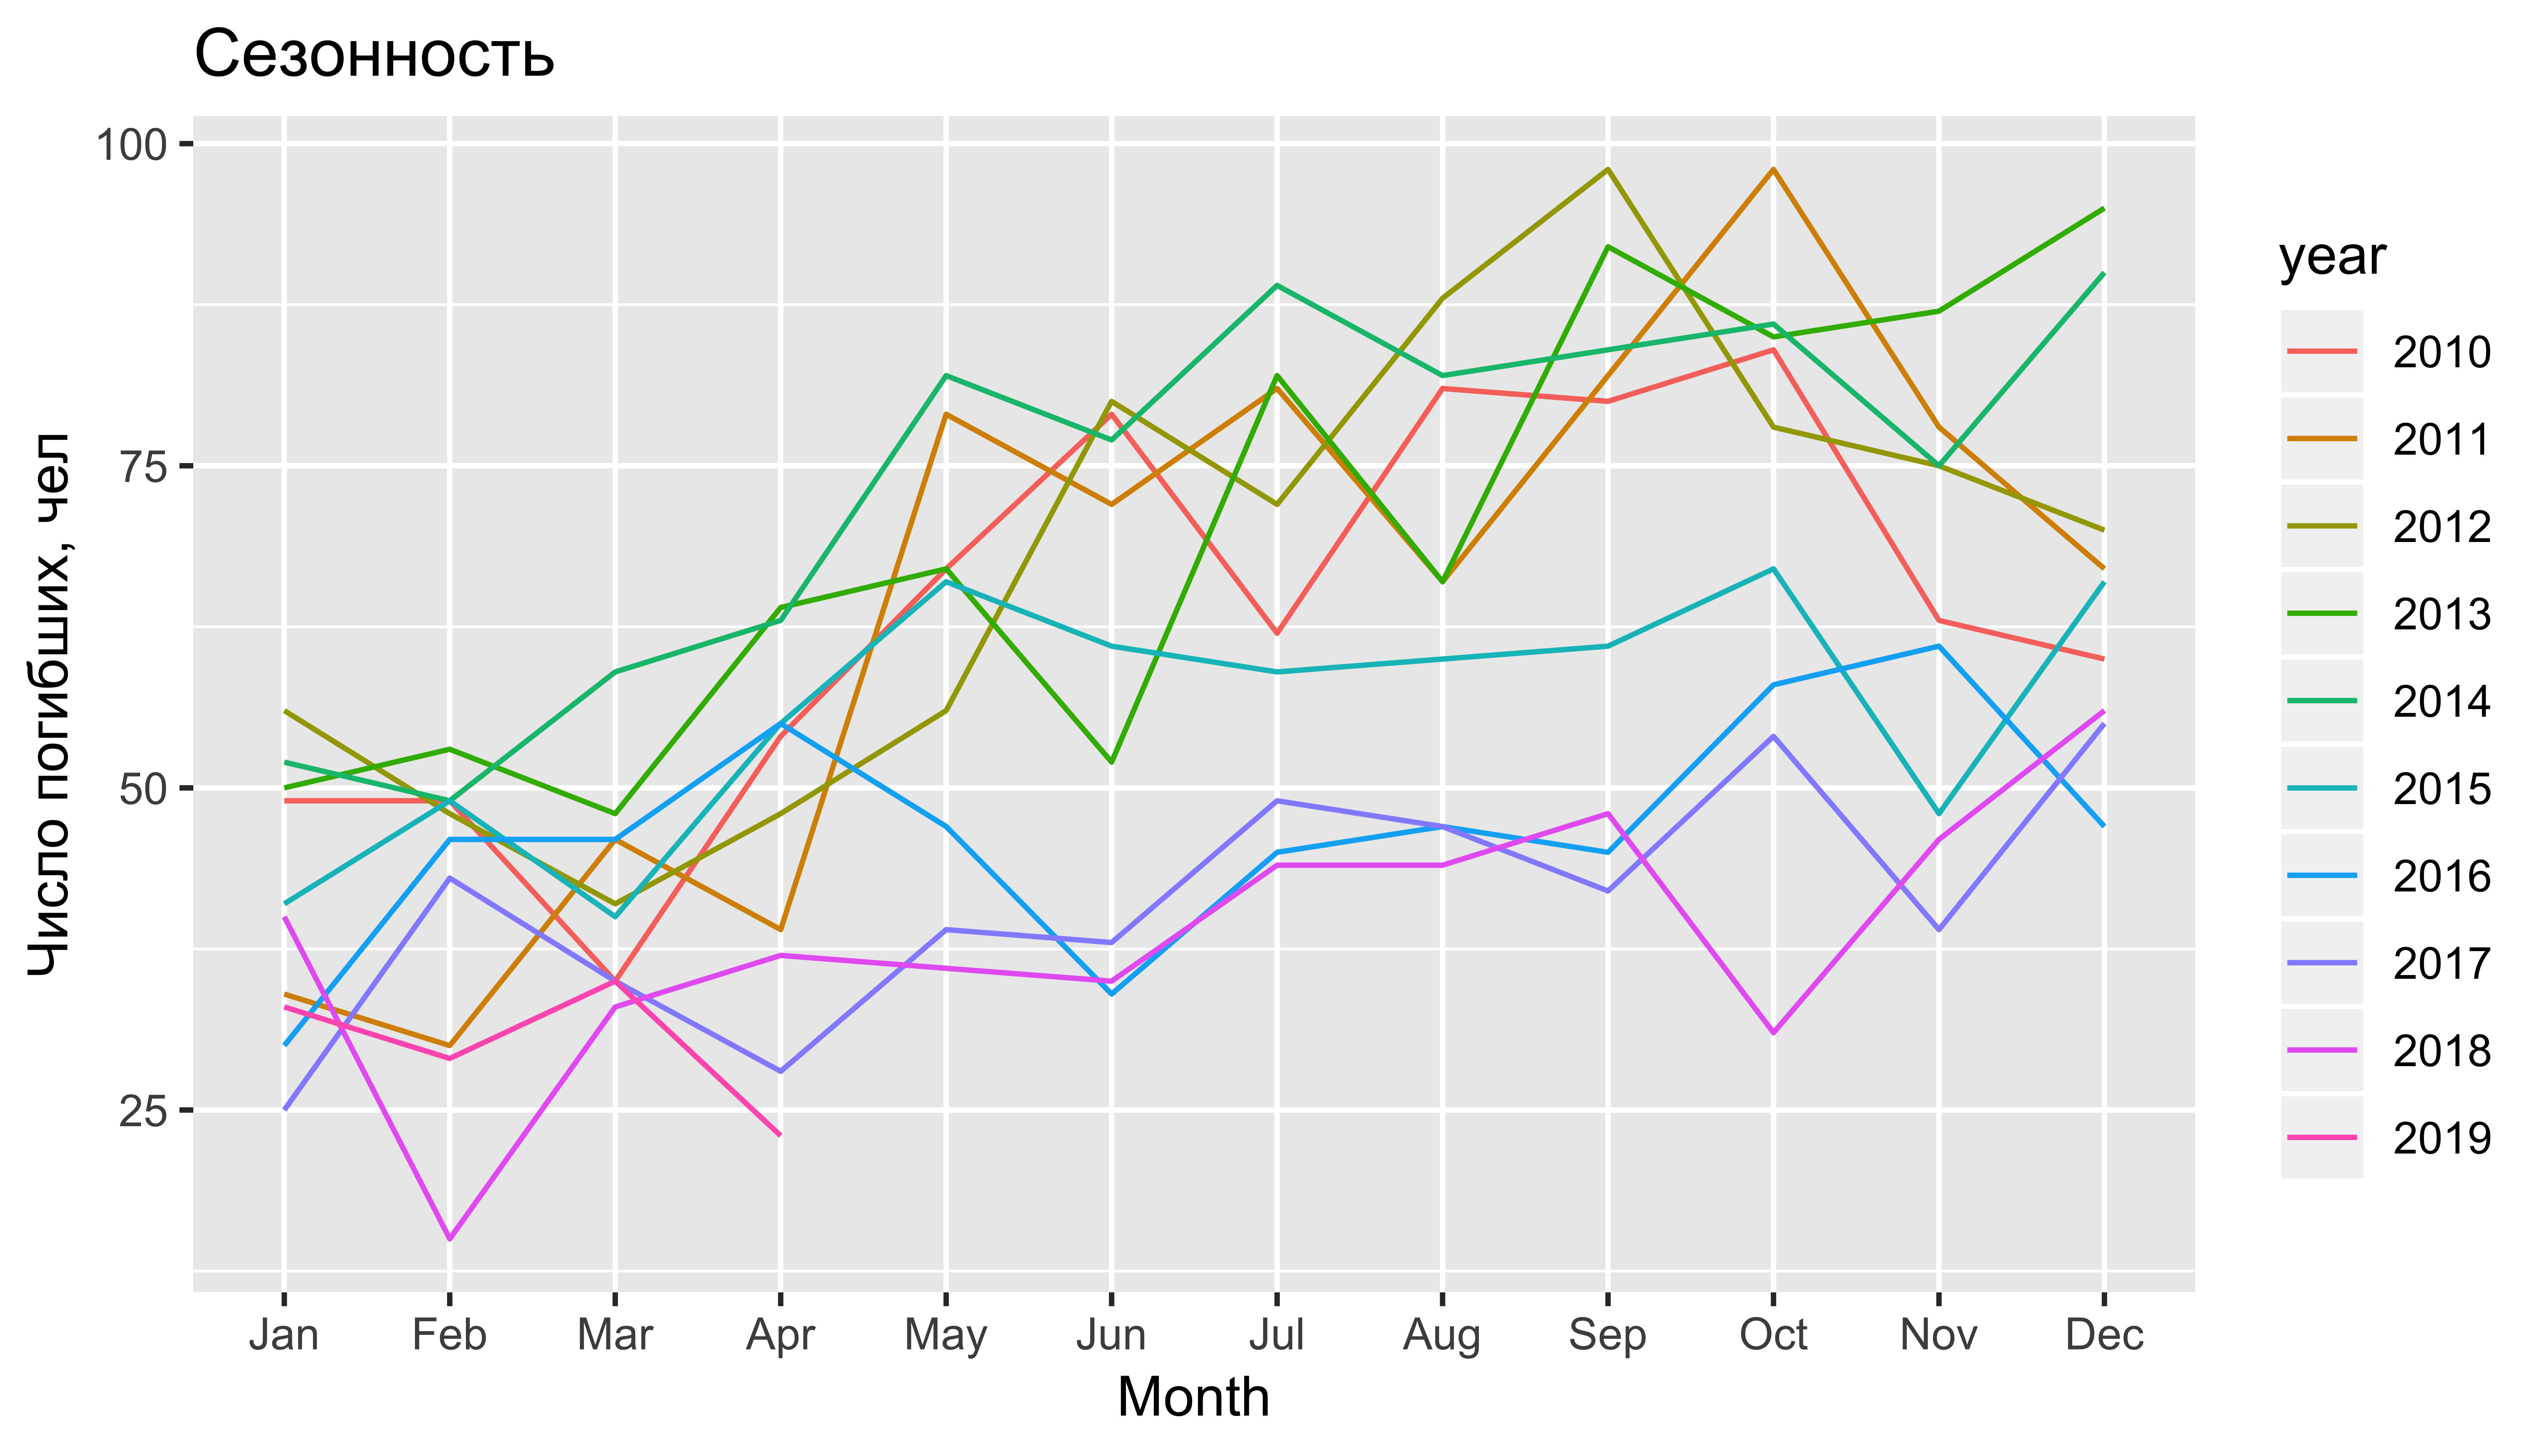
\includegraphics[width=\maxwidth]{figure/unnamed-chunk-2-1} 

}



\end{knitrout}
\end{figure}

\item Резкий сдвиг графика вниз в течение $2015$-ого года может быть структурным сдвигом, связанным с тем, что с 01.07.2015 ввели уголовную ответственнсть за вождение в нетрезвом виде. 

\item Визуально заметно, что дисперсия не постоянна, поэтому ряд не стационарен. Имеет смысл преобразовать данные. 

\end{enumerate}



Проделаю следующие шаги:

\begin{enumerate}

\item Через функцию BoxCox.lambda нахожу значение $\lambda$, которая подобрана функцией так, чтобы балансировать дисперсию. В нашем примере $\lambda$  равна $-0.01$, что довольно близко к $0$. $\lambda$, равная $0$ в преобразовании Бокса-Кокса, означает, что мы должны взять логарифм от ряда. 

\begin{knitrout}
\definecolor{shadecolor}{rgb}{0.969, 0.969, 0.969}\color{fgcolor}\begin{kframe}
\begin{verbatim}
## [1] -0.01222915
\end{verbatim}
\end{kframe}
\end{knitrout}

\begin{figure} [H]
\begin{knitrout}
\definecolor{shadecolor}{rgb}{0.969, 0.969, 0.969}\color{fgcolor}

{\centering 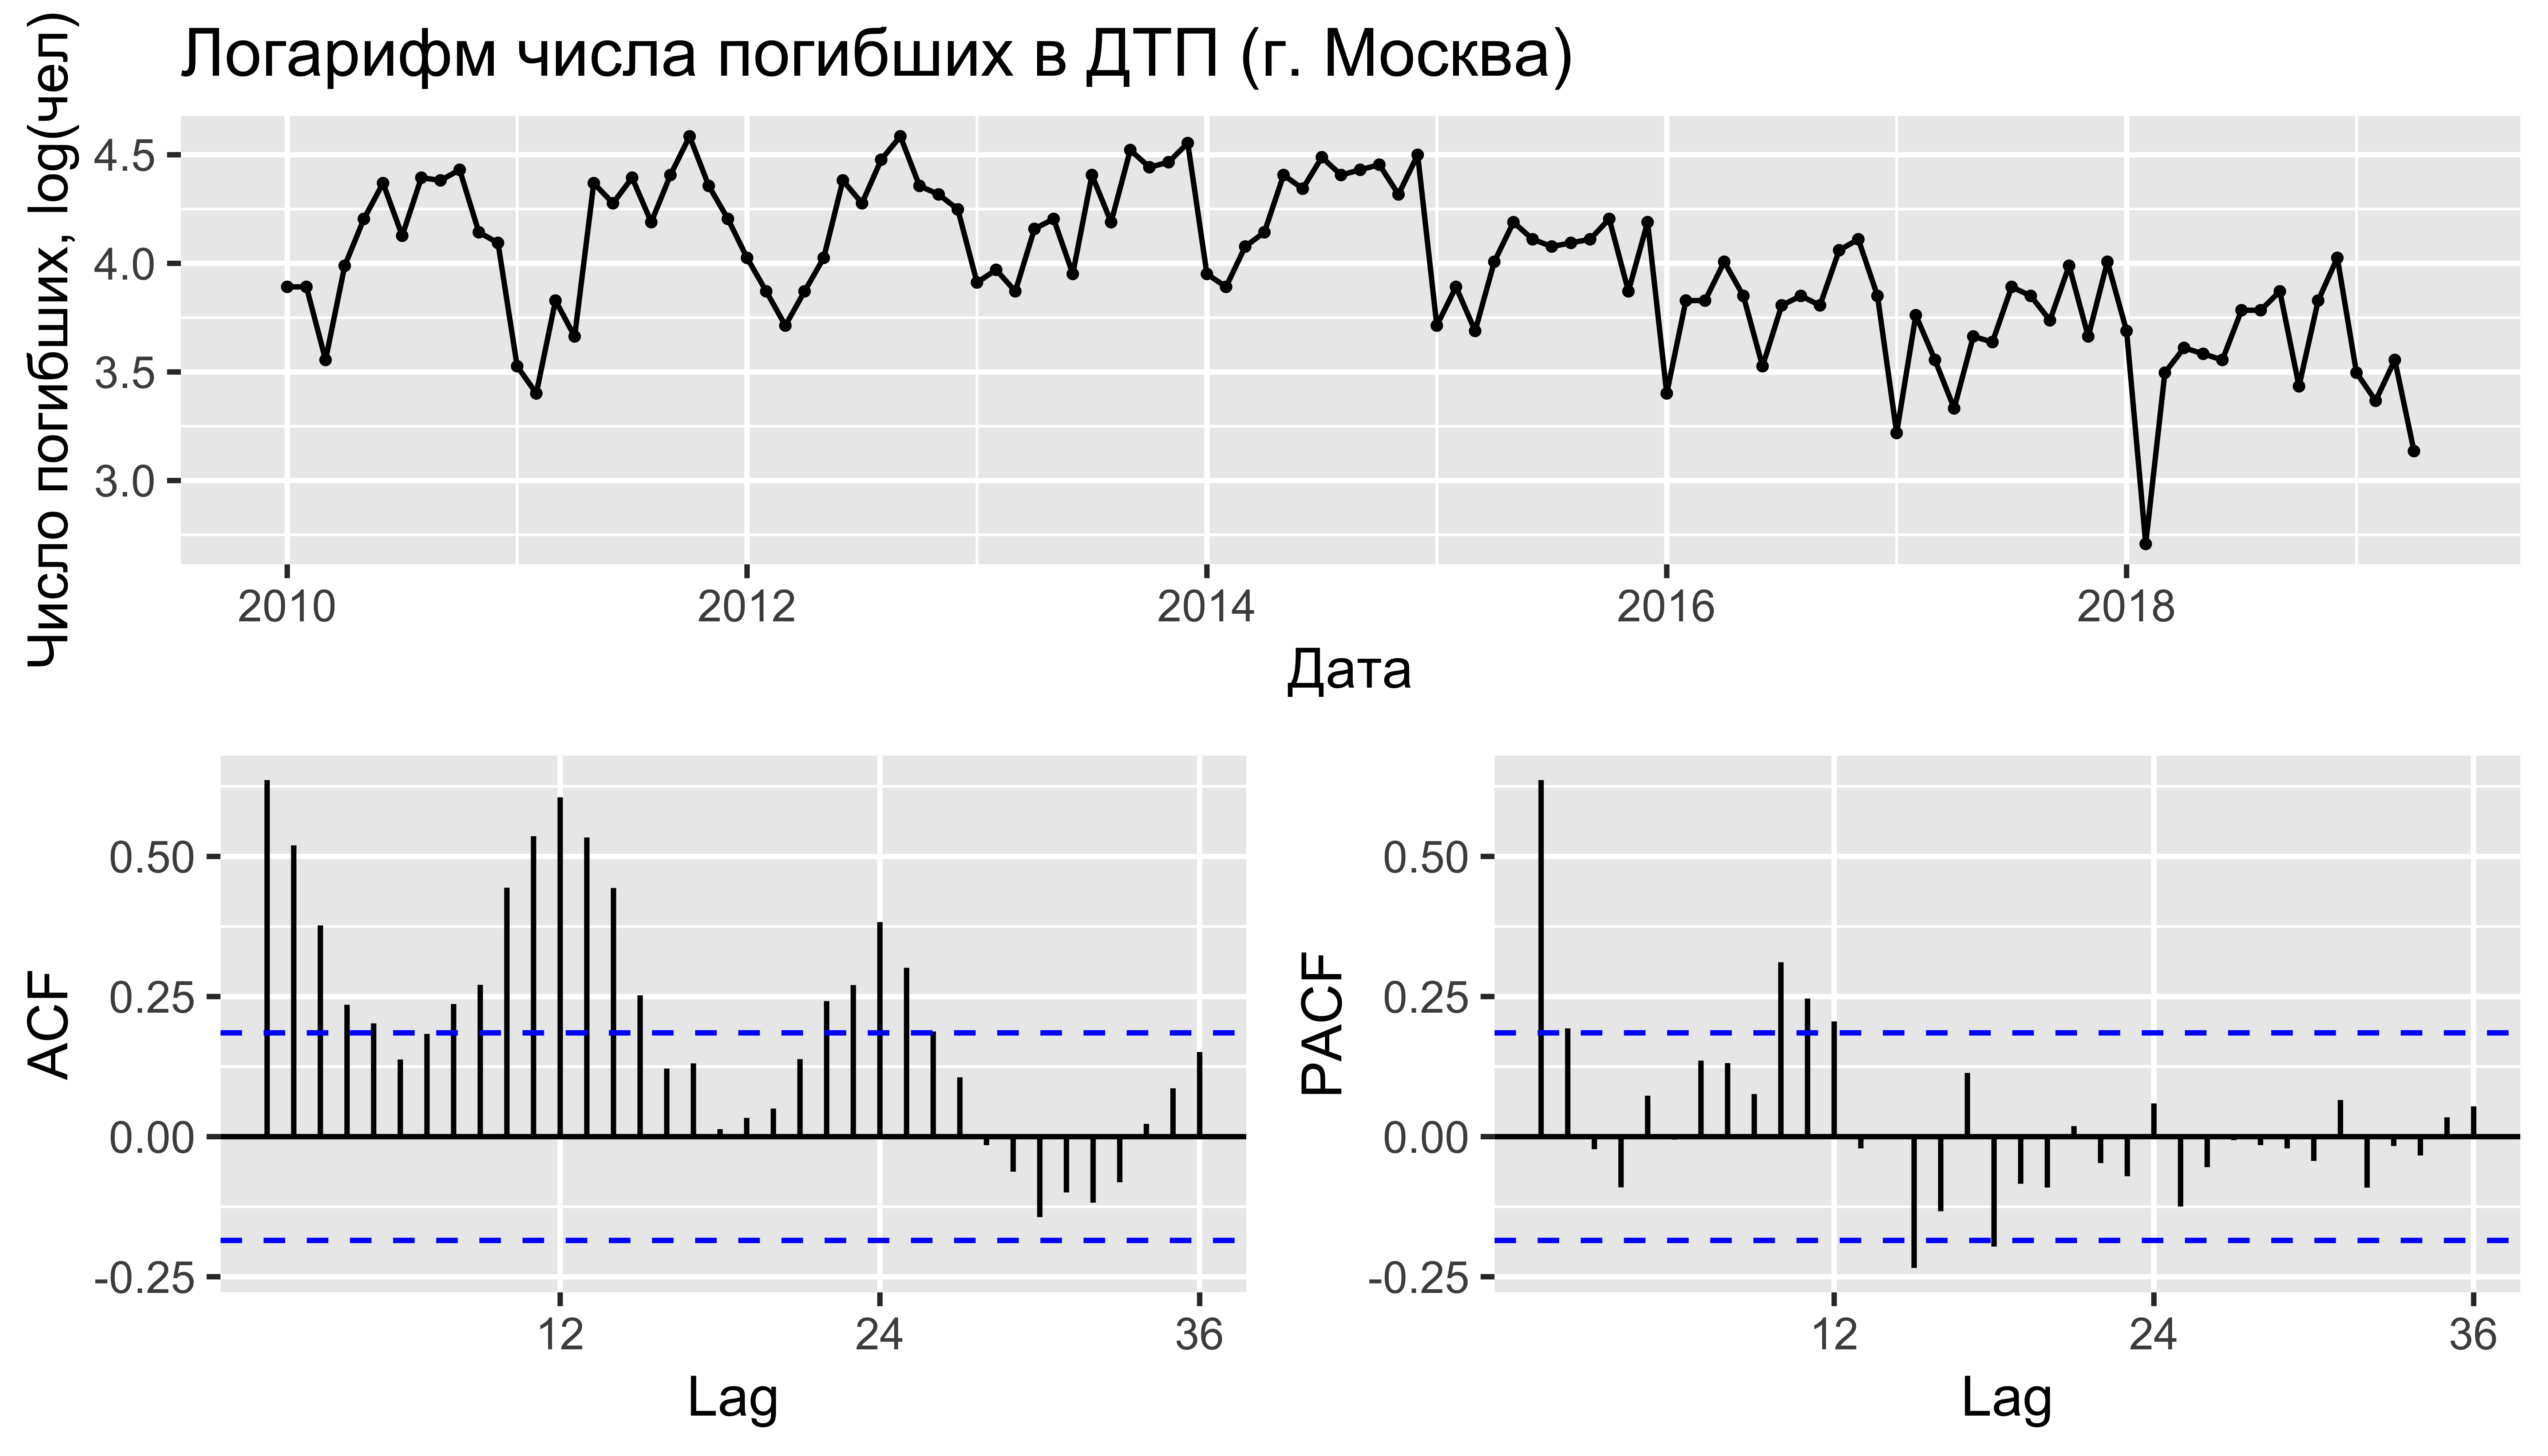
\includegraphics[width=\maxwidth]{figure/unnamed-chunk-5-1} 

}



\end{knitrout}
\end{figure}

\item Через HEGY тест проверяю наличие сезонного корня. Сезонный корень присутствует.

\begin{knitrout}
\definecolor{shadecolor}{rgb}{1, 1, 1}\color{fgcolor}\begin{kframe}
\begin{verbatim}
## 
## 	HEGY test for unit roots
## 
## data:  logdtp
## 
##         statistic p-value    
## t_1        0.4618  0.9804    
## t_2        -2.299  0.0158 *  
## F_3:4      1.2176  0.2962    
## F_5:6      2.5615  0.0788 .  
## F_7:8      5.9895  0.0031 ** 
## F_9:10     6.8748  0.0014 ** 
## F_11:12    5.0975   0.007 ** 
## F_2:12     4.7426   8e-04 ***
## F_1:12     4.4255  0.0025 ** 
## ---
## Signif. codes: 0 '***' 0.001 '**' 0.01 '*' 0.05 '.' 0.1 ' ' 1 
## 
## Deterministic terms: constant 
## Lag selection criterion and order: fixed, 0
## P-values: based on response surface regressions
## [1] 1
\end{verbatim}
\end{kframe}
\end{knitrout}

\item Беру разность с шагом $12$ (то есть diff(x,12)), чтобы убрать сезонность и прикинуть параметры модели.

\begin{figure}[H]
\begin{knitrout}
\definecolor{shadecolor}{rgb}{0.969, 0.969, 0.969}\color{fgcolor}

{\centering 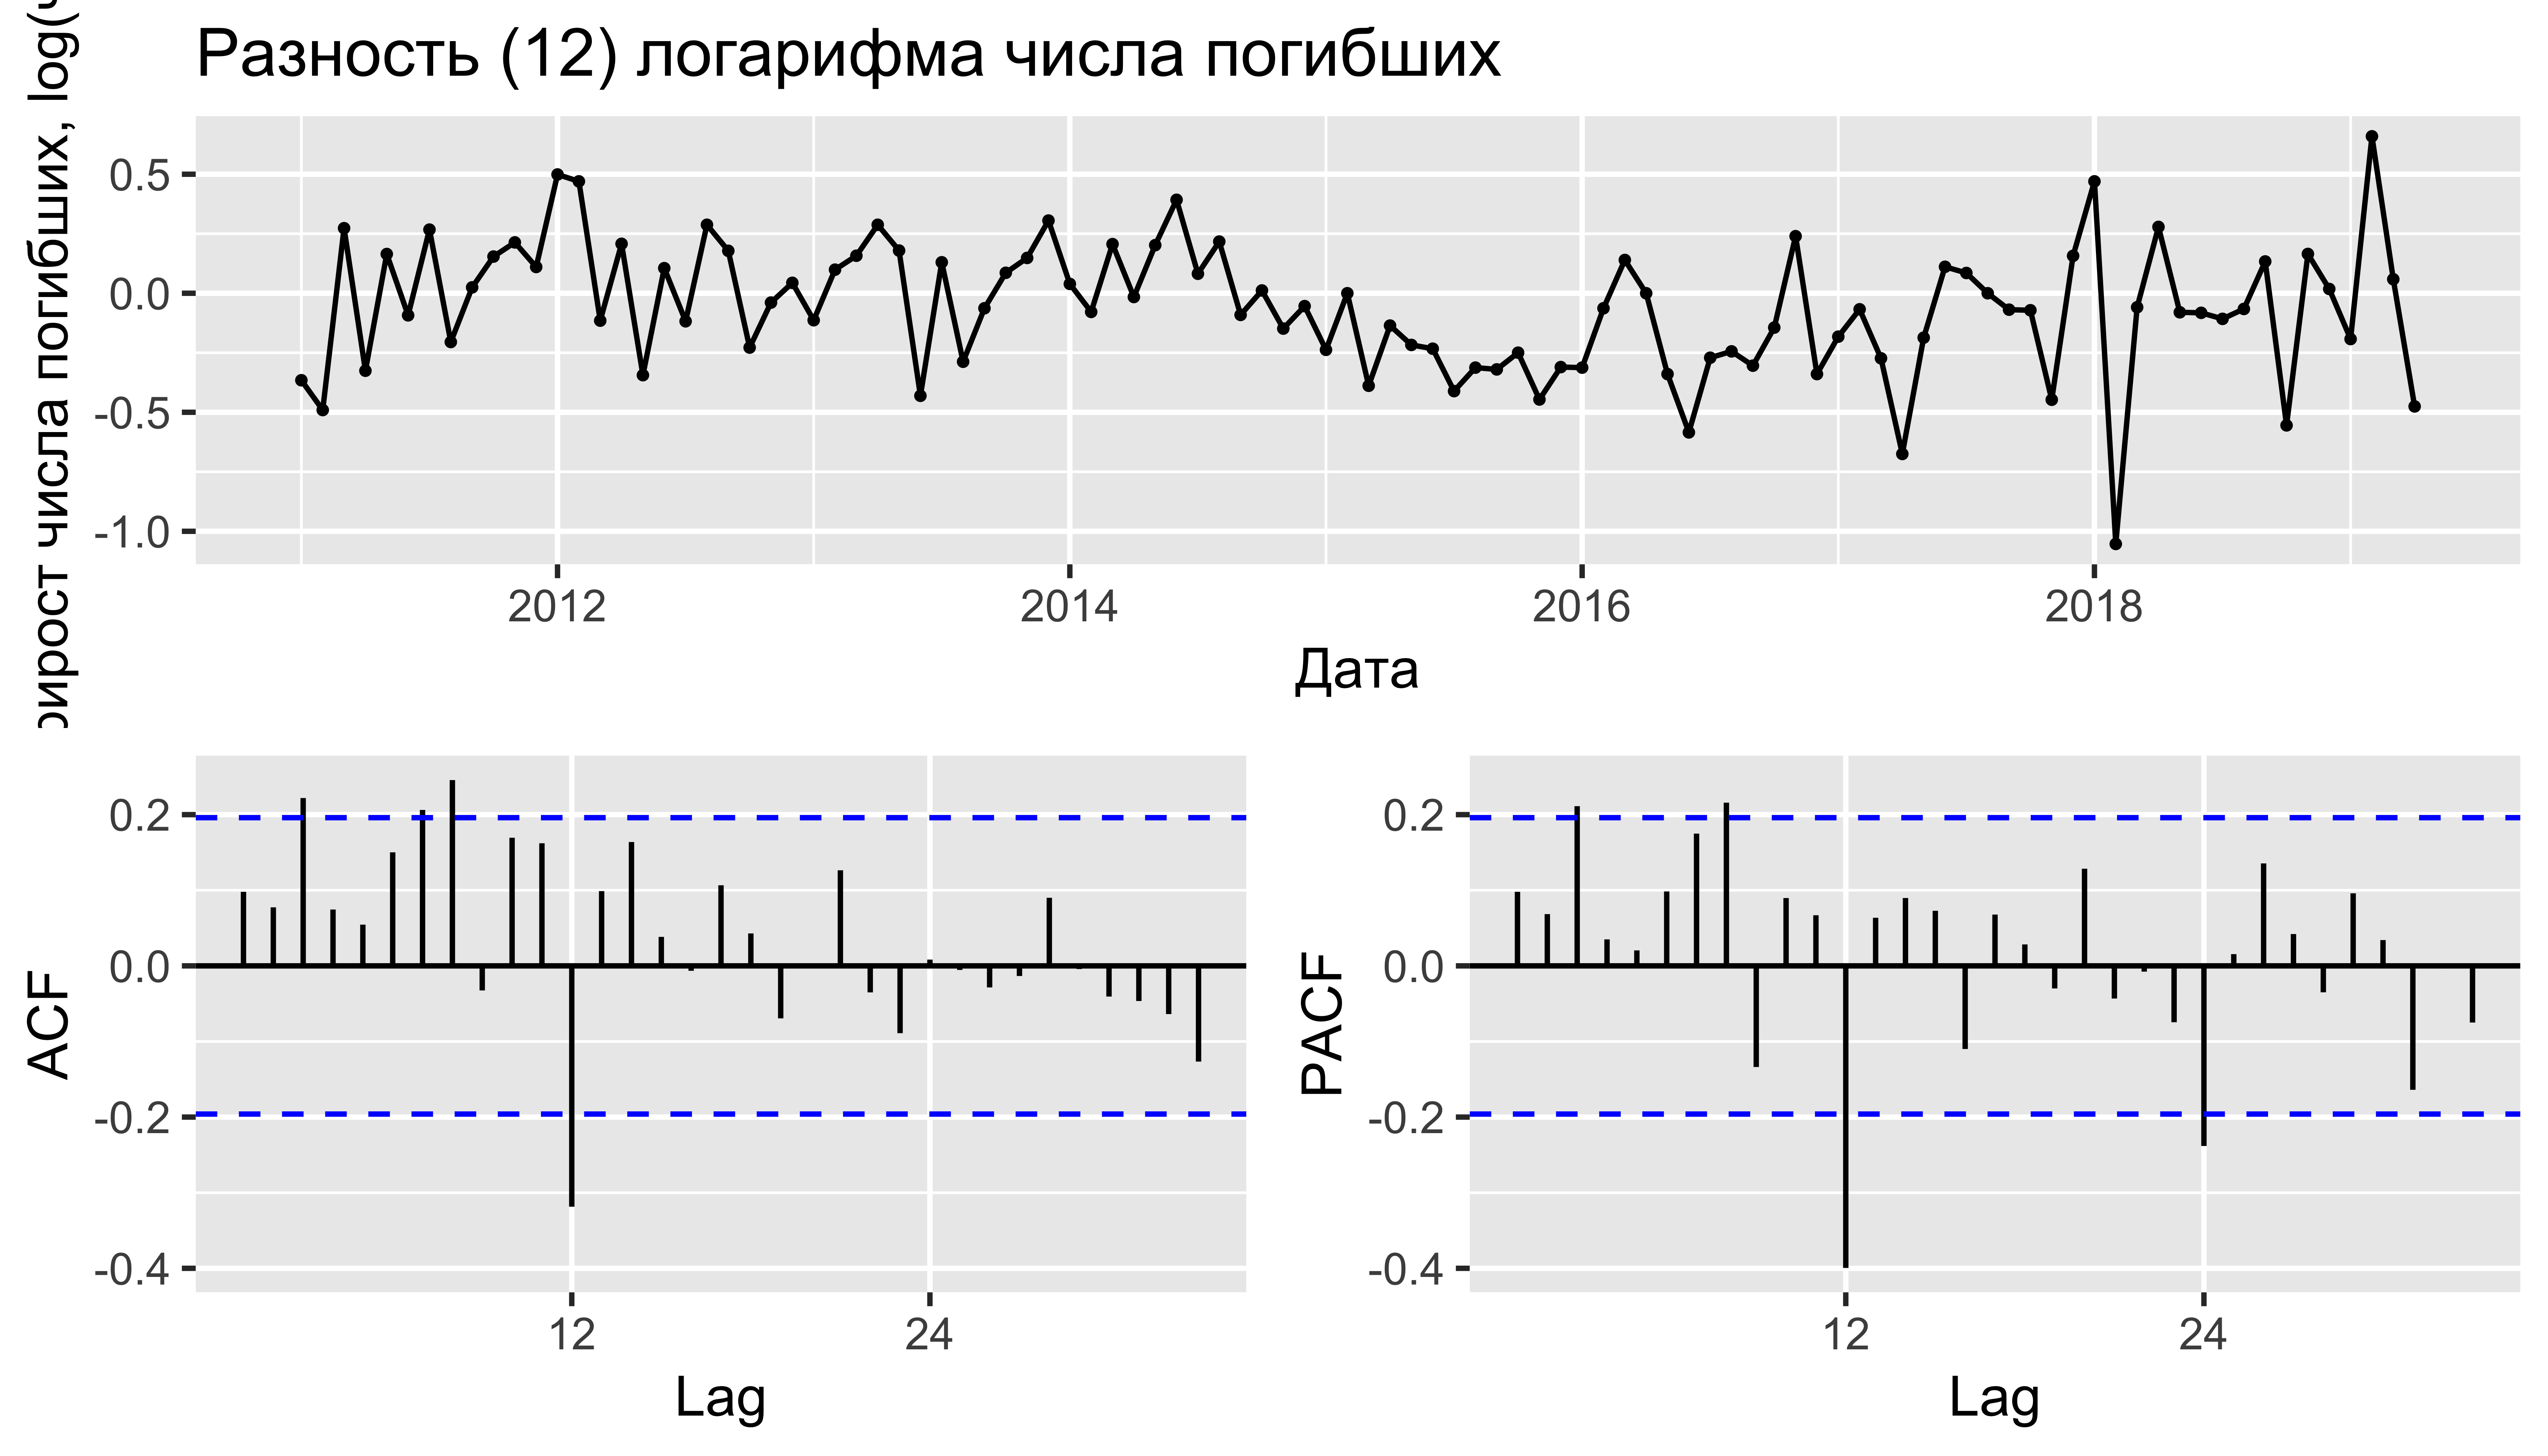
\includegraphics[width=\maxwidth]{figure/unnamed-chunk-7-1} 

}



\end{knitrout}
\end{figure}

\item Видно, что есть сезонный $MA(1)$. Имеет смысл проверить несколько моделей и сравнить их с тем, что предлагает автоматический подбор модели. 

\item Проверяю данные с взятой сезонной разностью на наличие единичного корня (если гипотеза о нем отвергается, то ряд стационарен). Критическое значение tao $5 \% = - 1.95 \Rightarrow$ гипотеза отвергается и ряд стационарен. 

\begin{knitrout}
\definecolor{shadecolor}{rgb}{1, 1, 1}\color{fgcolor}\begin{kframe}
\begin{verbatim}
## 
## ############################################################### 
## # Augmented Dickey-Fuller Test Unit Root / Cointegration Test # 
## ############################################################### 
## 
## The value of the test statistic is: -6.0112
\end{verbatim}
\end{kframe}
\end{knitrout}
\end{enumerate}


%%%%%%%%%%%%%%%%%%%%%%%%%%%%%%%%%%%%%%%%%%%%%%%%%%%%%%%%%%%%%%%%%%%%%%%%%%%%%%%%%%%%%%%%%%%%%%%%%%%%%%%%%
\subsection{Проверка моделей}

Теперь проверяю несколько моделей. Для всех из них данные преобразованы с $\lambda = -0.01$, а затем через параметр biasadj = TRUE происходит обратное преобразование для прогнозирования данных в подходящих единицах измерения (чел).

\begin{enumerate}
\item ARIMA[0,0,0][0,1,1][12] с дамми-переменной 
\item ARIMA[1,0,0][0,1,1][12] с дамми-переменной 
\item auto-arima [1,0,1][0,1,1][12] с дамми-переменной 
\item ARIMA[1,0,1][0,1,1][12]  
\item auto-arima [0,1,1][0,1,1][12] 
\item ets
\end{enumerate}

Ниже привожу пять вариаций моделей ARIMA, где указаны коэффициенты и штрафные критерии.




\begin{table}[h]
\begin{center}
\begin{tabular}{l c c c c c }
\hline
 & *[1,0,1]+D & [0,0,0]+D & [1,0,0]+D & *[0,1,1] & [1,0,1] \\
\hline
ar1            & $0.98$   &          & $0.16$   &          & $0.99$   \\
               & $(0.03)$ &          & $(0.10)$ &          & $(0.01)$ \\
ma1            & $-0.87$  &          &          & $-0.81$  & $-0.81$  \\
               & $(0.05)$ &          &          & $(0.05)$ & $(0.05)$ \\
sma1           & $-0.79$  & $-0.80$  & $-0.83$  & $-0.77$  & $-0.77$  \\
               & $(0.13)$ & $(0.16)$ & $(0.18)$ & $(0.12)$ & $(0.12)$ \\
xreg           & $-0.28$  & $-0.42$  & $-0.42$  &          &          \\
               & $(0.11)$ & $(0.04)$ & $(0.05)$ &          &          \\
\hline
AIC            & -21.99   & -17.15   & -17.57   & -17.49   & -18.33   \\
AICc           & -21.35   & -16.90   & -17.15   & -17.24   & -17.90   \\
BIC            & -8.97    & -9.33    & -7.15    & -9.70    & -7.91    \\
Log Likelihood & 16.00    & 11.57    & 12.79    & 11.74    & 13.16    \\
\hline
\multicolumn{6}{l}{\scriptsize{*=авто модель, D=дамми, сезонная часть для всех одинакова}}
\end{tabular}
\caption{Вариации моделей ARIMA}
\label{table:coefficients}
\end{center}
\end{table}



По критерию AICc модель [1,0,1][0,1,1][12]+D оказывается лучше других. 


\begin{figure}[H]
\begin{knitrout}
\definecolor{shadecolor}{rgb}{0.969, 0.969, 0.969}\color{fgcolor}

{\centering 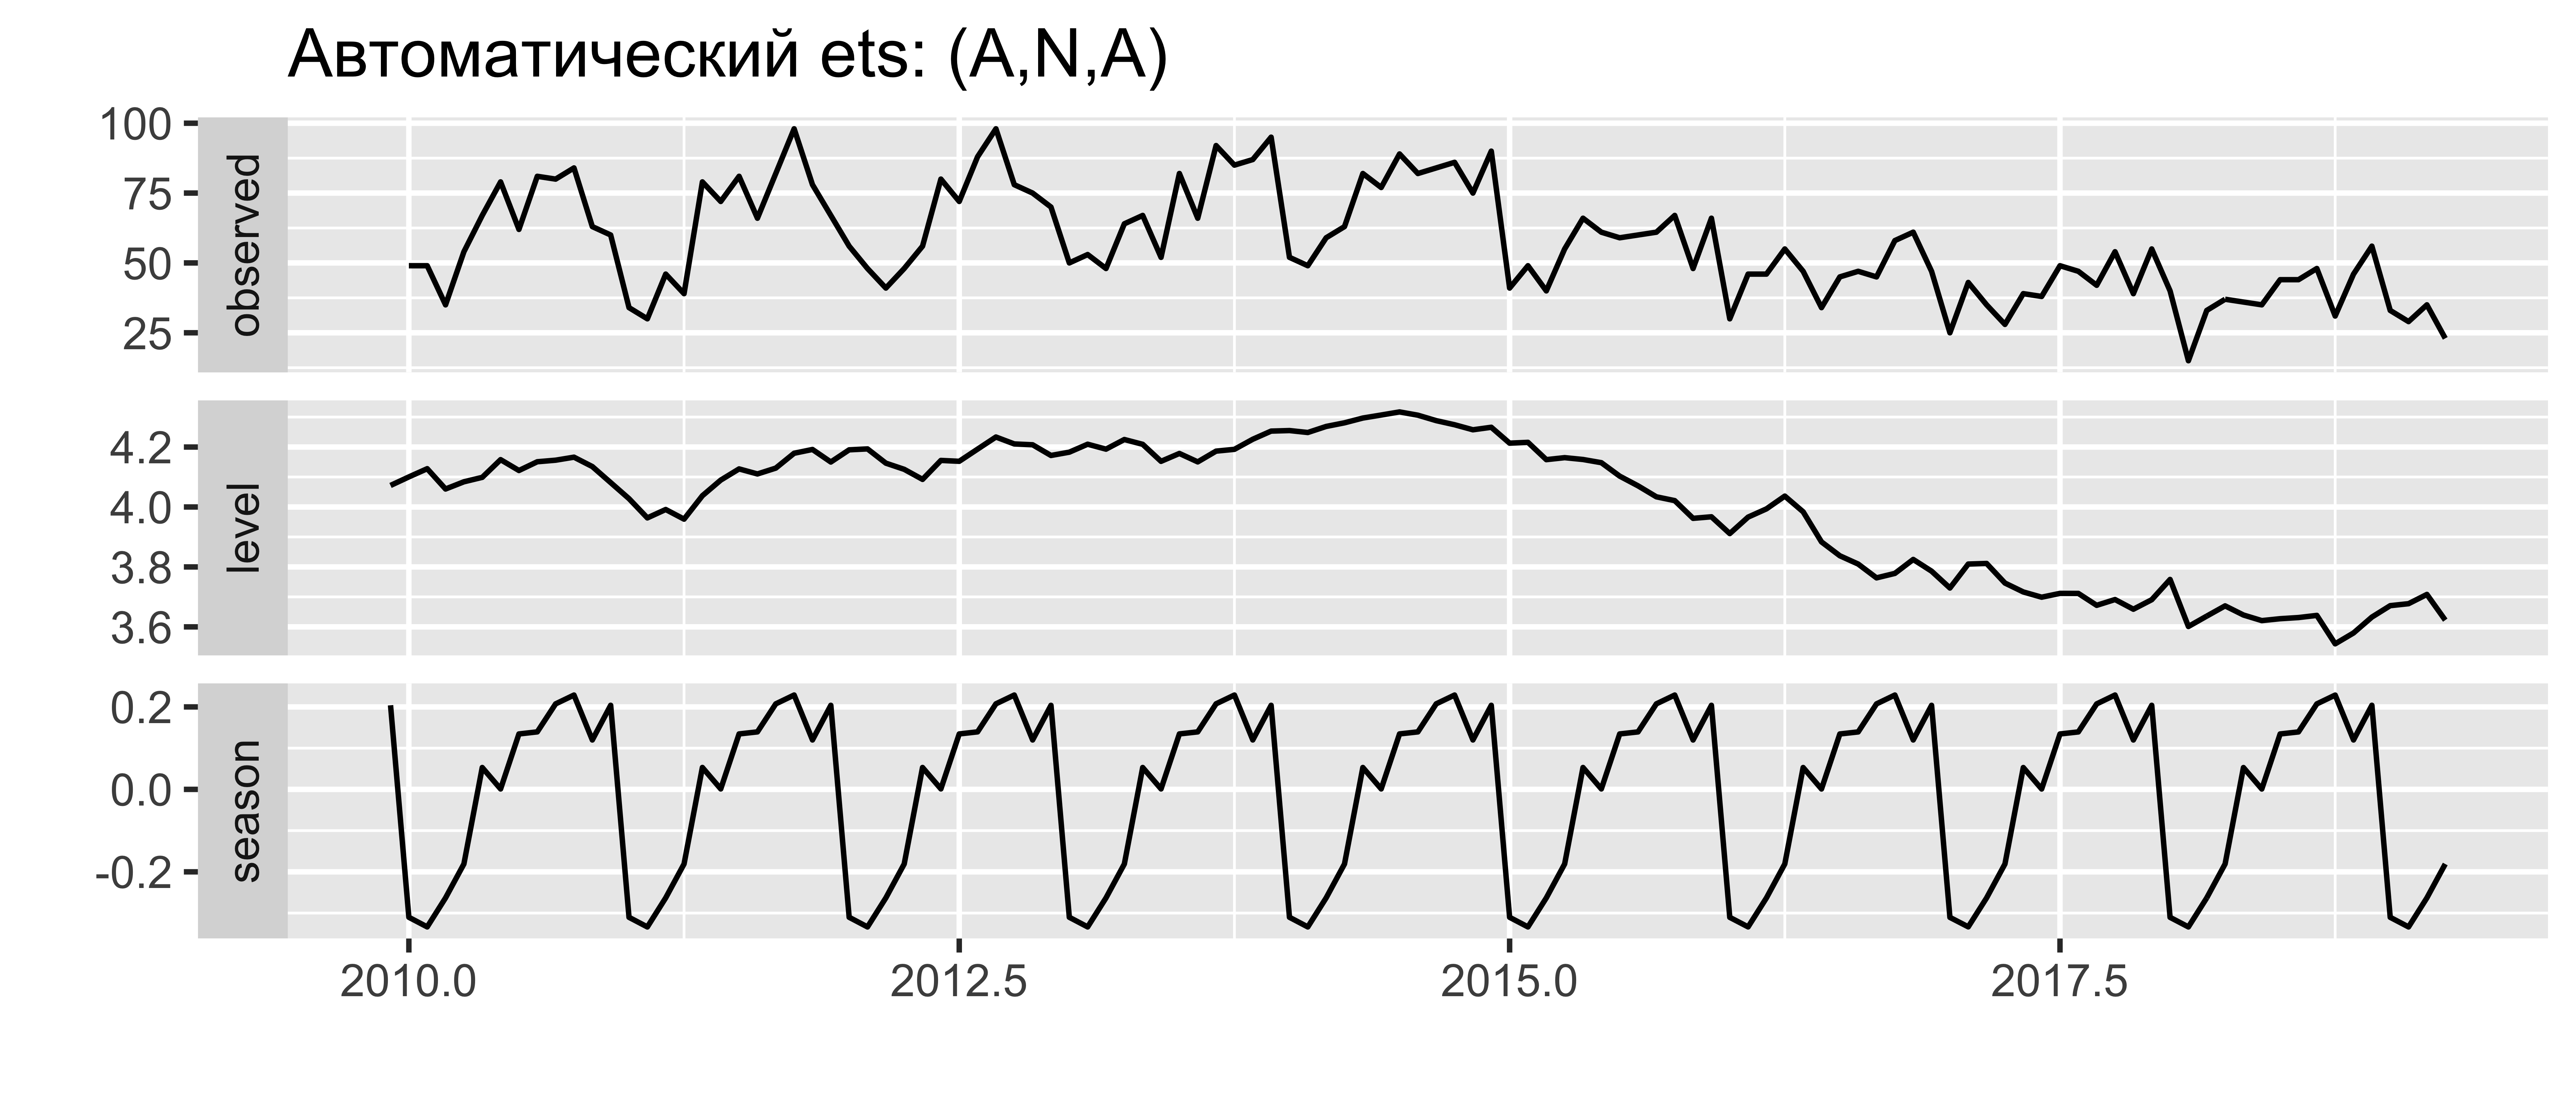
\includegraphics[width=\maxwidth]{figure/unnamed-chunk-12-1} 

}



\end{knitrout}
\end{figure}
Коэффициенты ETS модели:
\begin{knitrout}
\definecolor{shadecolor}{rgb}{1, 1, 1}\color{fgcolor}\begin{kframe}
\begin{verbatim}
## ETS(A,N,A) 
## 
## Call:
##  ets(y = dtp_ts, lambda = 0, biasadj = TRUE) 
## 
##   Box-Cox transformation: lambda= 0 
## 
##   Smoothing parameters:
##     alpha = 0.219 
##     gamma = 3e-04 
## 
##   Initial states:
##     l = 4.0718 
##     s = 0.204 0.1199 0.2288 0.2074 0.1394 0.1345
##            9e-04 0.0529 -0.1809 -0.263 -0.3336 -0.3103
## 
##   sigma:  0.1998
## 
##      AIC     AICc      BIC 
## 182.7611 187.7611 223.5385
\end{verbatim}
\end{kframe}
\end{knitrout}



Создав тренировочный массив из 89 наблюдений (до 05.2017), я прогнозирую на 23 месяца вперед и сравниваю с актульными данными. 

\begin{table}[H]
\centering
\begin{tabular}{rrrrrrrrrr}
  \hline
 & ME & RMSE & MAE & MPE & MAPE & MASE & ACF1 & Theil's U \\ 
  \hline
A: Training set & 0.11 & 9.65 & 7.50 & -2.22 & 13.60 & 0.58 & -0.11 &  \\ 
   Test set & -7.05 & 11.19 & 8.30 & -24.20 & 27.47 & 0.65 & -0.15 & 0.72 \\ 
   \hline
   B: Training set & 0.89 & 9.76 & 7.71 & -1.09 & 13.99 & 0.60 & 0.14 &  \\ 
   Test set & -7.75 & 11.53 & 8.98 & -25.77 & 28.95 & 0.70 & -0.15 & 0.74 \\ 
   \hline
  C: Training set & 0.53 & 9.72 & 7.74 & -1.58 & 13.89 & 0.60 & -0.15 &  \\ 
   Test set & -7.57 & 11.45 & 8.79 & -25.30 & 28.50 & 0.68 & -0.15 & 0.73 \\ 
   \hline
  D: Training set & -1.73 & 10.65 & 7.96 & -5.09 & 14.43 & 0.62 & 0.01 &  \\ 
  Test set & 1.74 & 8.26 & 6.69 & -1.10 & 20.65 & 0.52 & -0.25 & 0.52 \\ 
   \hline
   E: Training set & -1.20 & 10.74 & 7.88 & -3.78 & 13.82 & 0.61 & 0.04 &  \\ 
   Test set & 5.92 & 10.00 & 8.54 & 10.38 & 23.58 & 0.66 & -0.20 & 0.67 \\ 
   \hline
   ETS: Training set & -1.12 & 9.56 & 8.14 & -4.40 & 14.56 & 0.63 & 0.00 &  \\ 
   Test set & -2.80 & 8.48 & 6.55 & -12.31 & 21.10 & 0.51 & -0.13 & 0.54 \\ 
   \hline
\end{tabular}
\caption{Характеристики различных вариантов модели} 
\end{table}

Выделю отдельно RMSE: 
\begin{enumerate}
\item RMSE=11.19 для модели A: *[1,0,1][0,1,1][12]+D
\item RMSE=11.53 для модели B: [0,0,0][0,1,1][12]+D
\item RMSE=11.45 для модели C: [1,0,0][0,1,1][12]+D
\item RMSE=8.26 для модели D: [1,0,1][0,1,1][12]
\item RMSE=10.00 для модели E: *[0,1,1][0,1,1][12]
\item RMSE=8.48 для модели ETS. 
\end{enumerate}

Графики: синяя линия - прогноз, черная - истинные значения. 

\begin{minipage}[t]{0.5\textwidth}
\begin{figure}[H]
\begin{knitrout}
\definecolor{shadecolor}{rgb}{0.969, 0.969, 0.969}\color{fgcolor}

{\centering 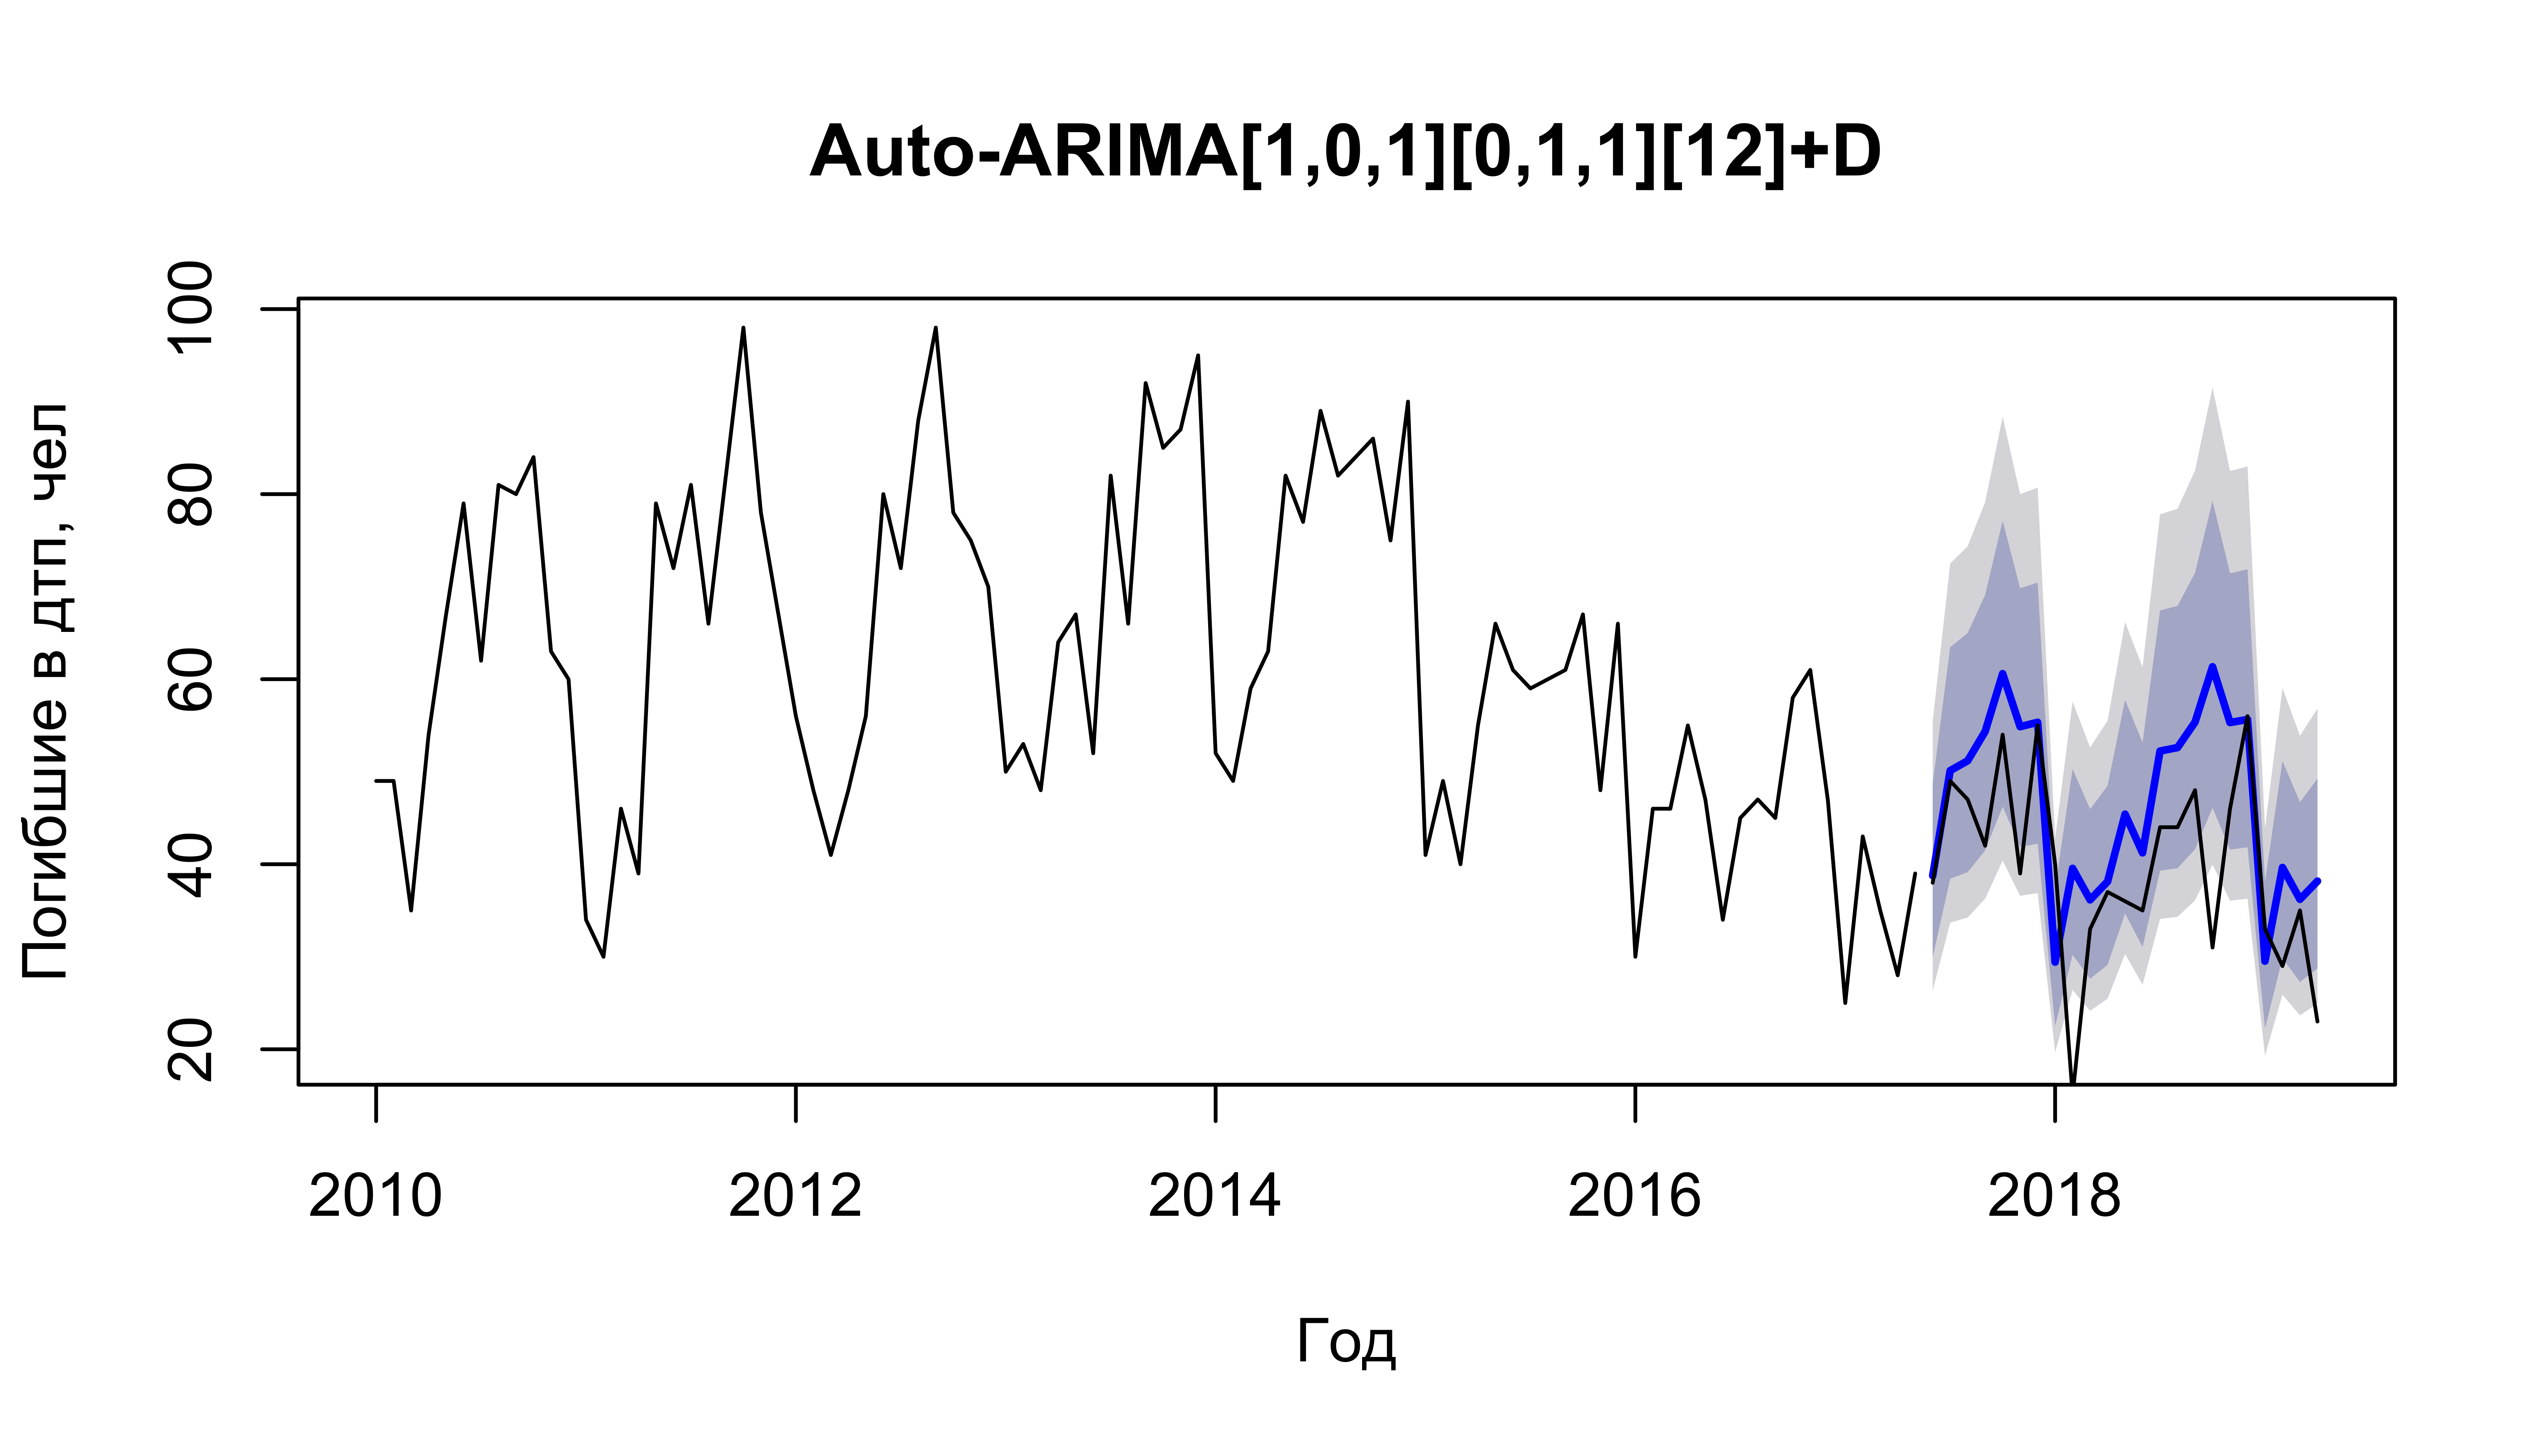
\includegraphics[width=\maxwidth]{figure/unnamed-chunk-15-1} 

}



\end{knitrout}
\end{figure}
\end{minipage}

\begin{minipage}[t]{0.5\textwidth}
\begin{figure}[H]
\begin{knitrout}
\definecolor{shadecolor}{rgb}{0.969, 0.969, 0.969}\color{fgcolor}

{\centering 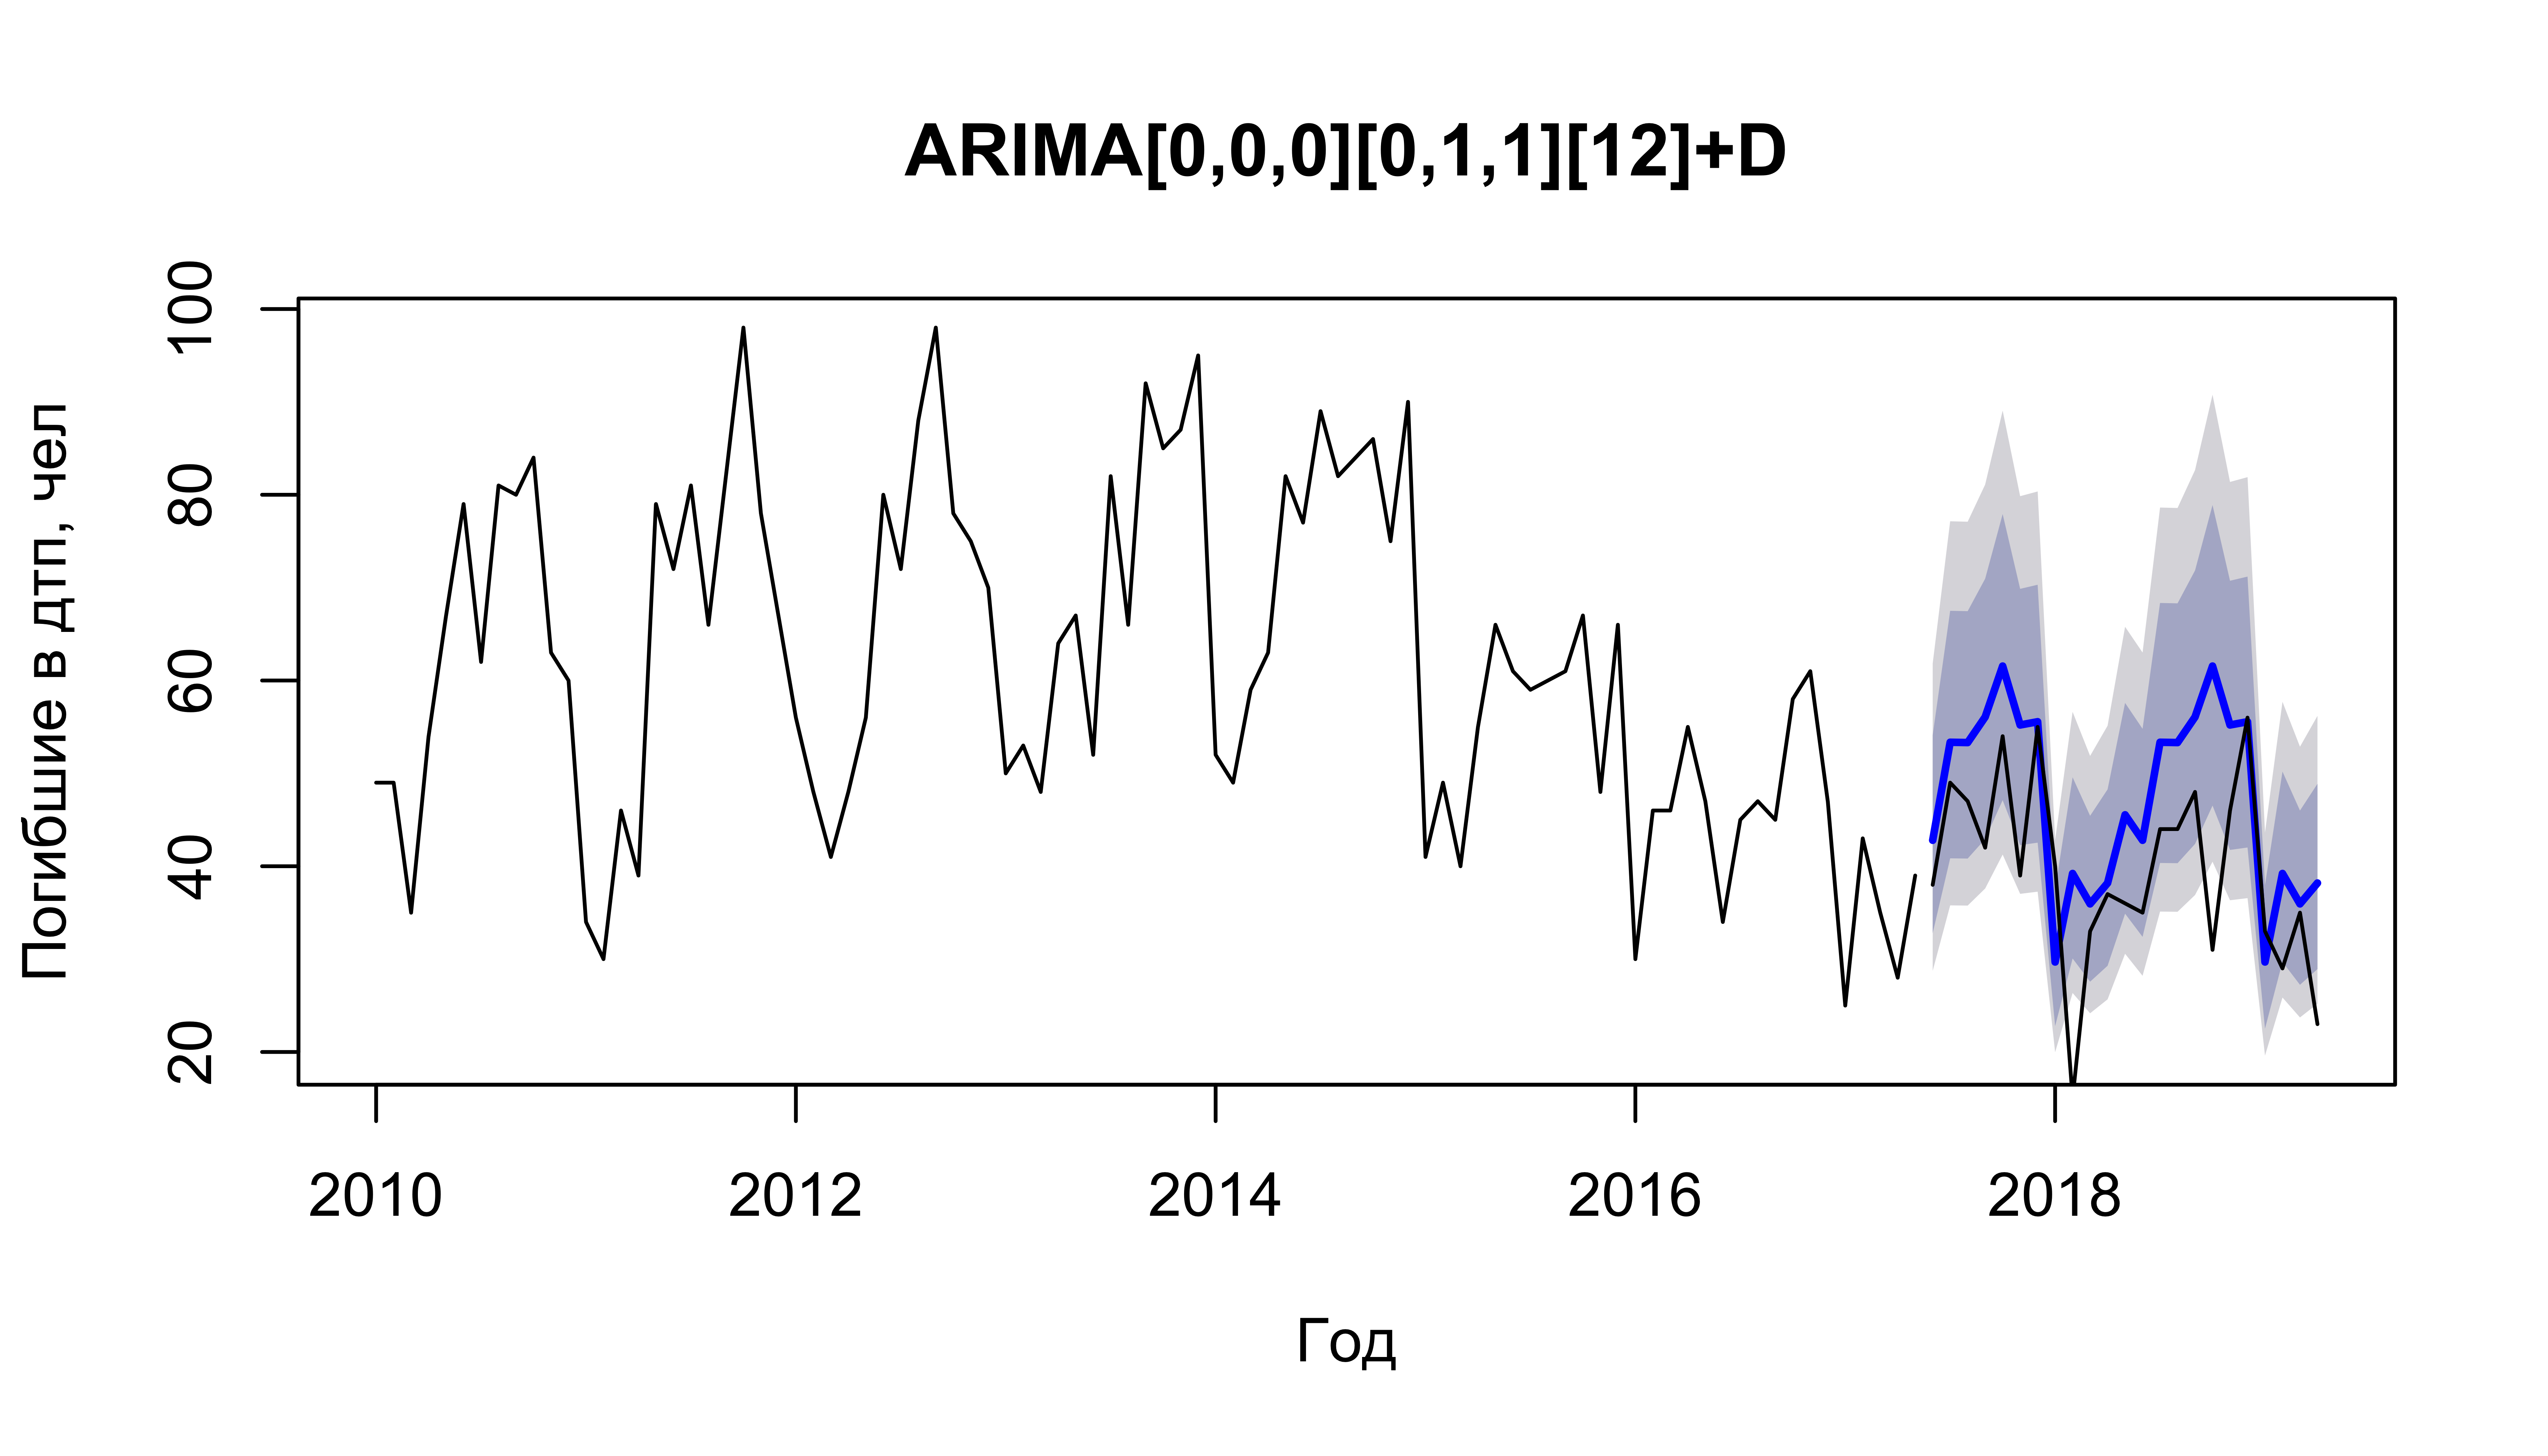
\includegraphics[width=\maxwidth]{figure/unnamed-chunk-16-1} 

}



\end{knitrout}
\end{figure}
\end{minipage}

\begin{minipage}[t]{0.5\textwidth}
\begin{figure}[H]
\begin{knitrout}
\definecolor{shadecolor}{rgb}{0.969, 0.969, 0.969}\color{fgcolor}

{\centering 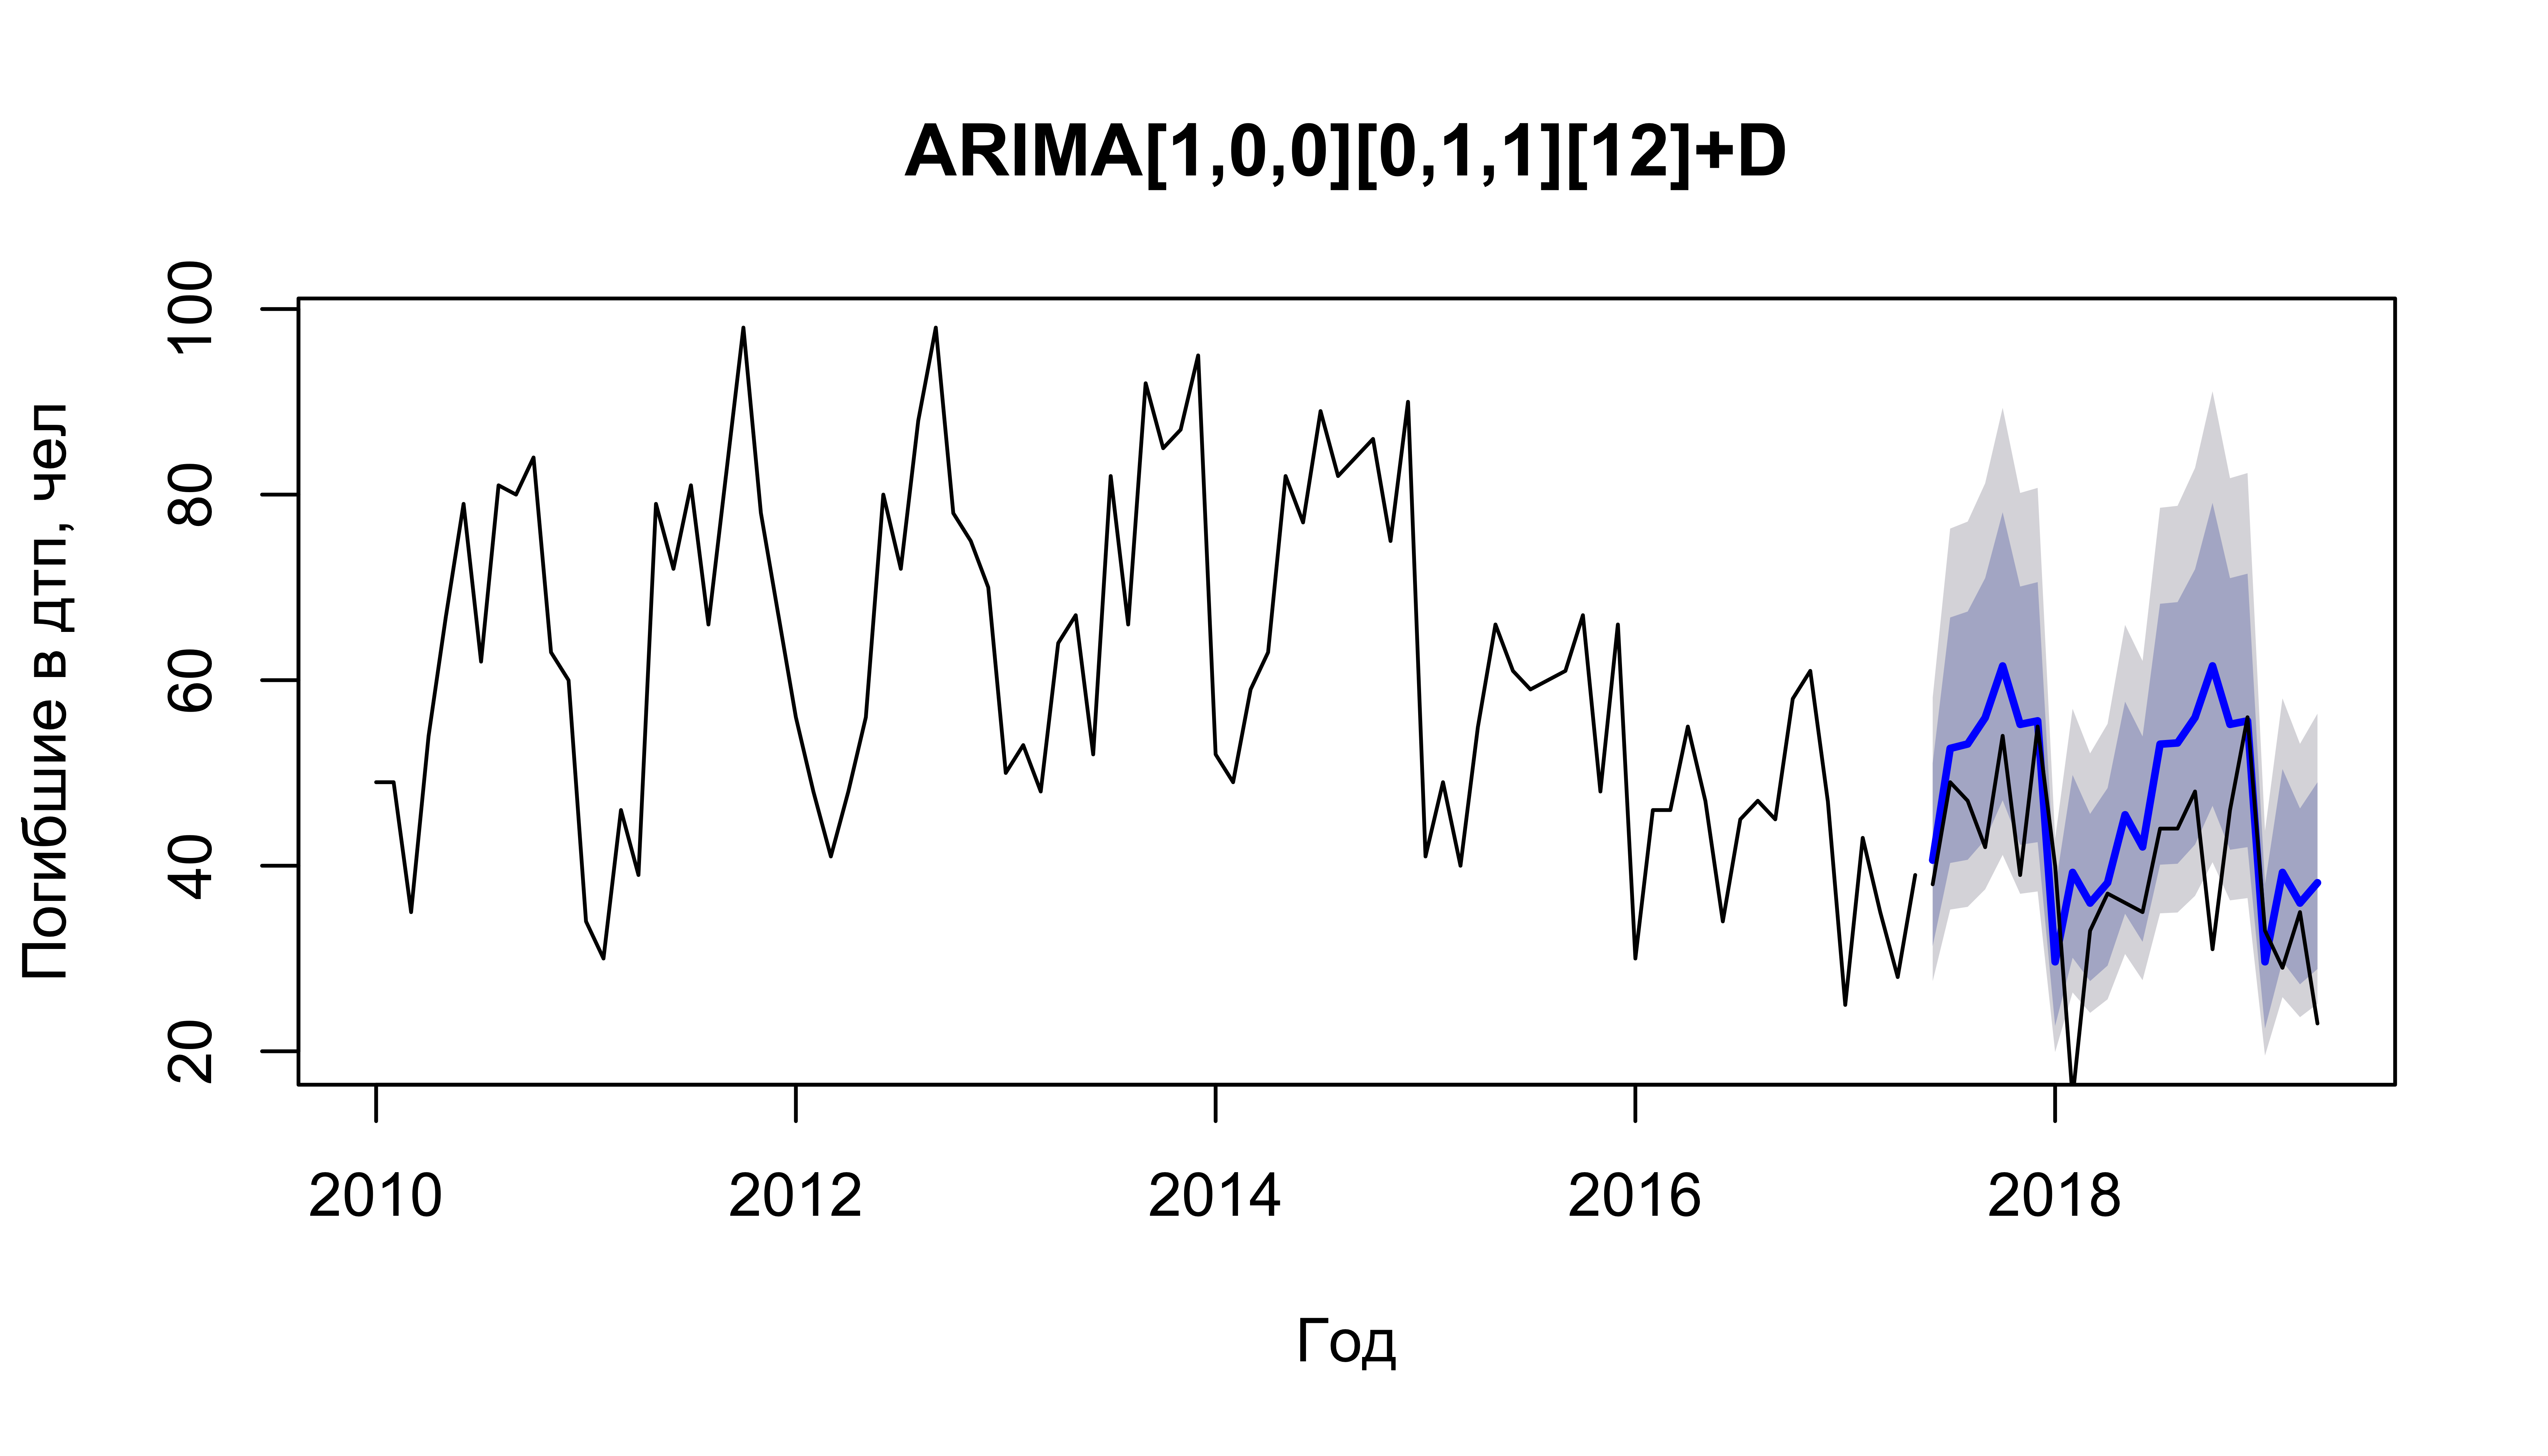
\includegraphics[width=\maxwidth]{figure/unnamed-chunk-17-1} 

}



\end{knitrout}
\end{figure}
\end{minipage}

\begin{minipage}[t]{0.5\textwidth}
\begin{figure}[H]
\begin{knitrout}
\definecolor{shadecolor}{rgb}{0.969, 0.969, 0.969}\color{fgcolor}

{\centering 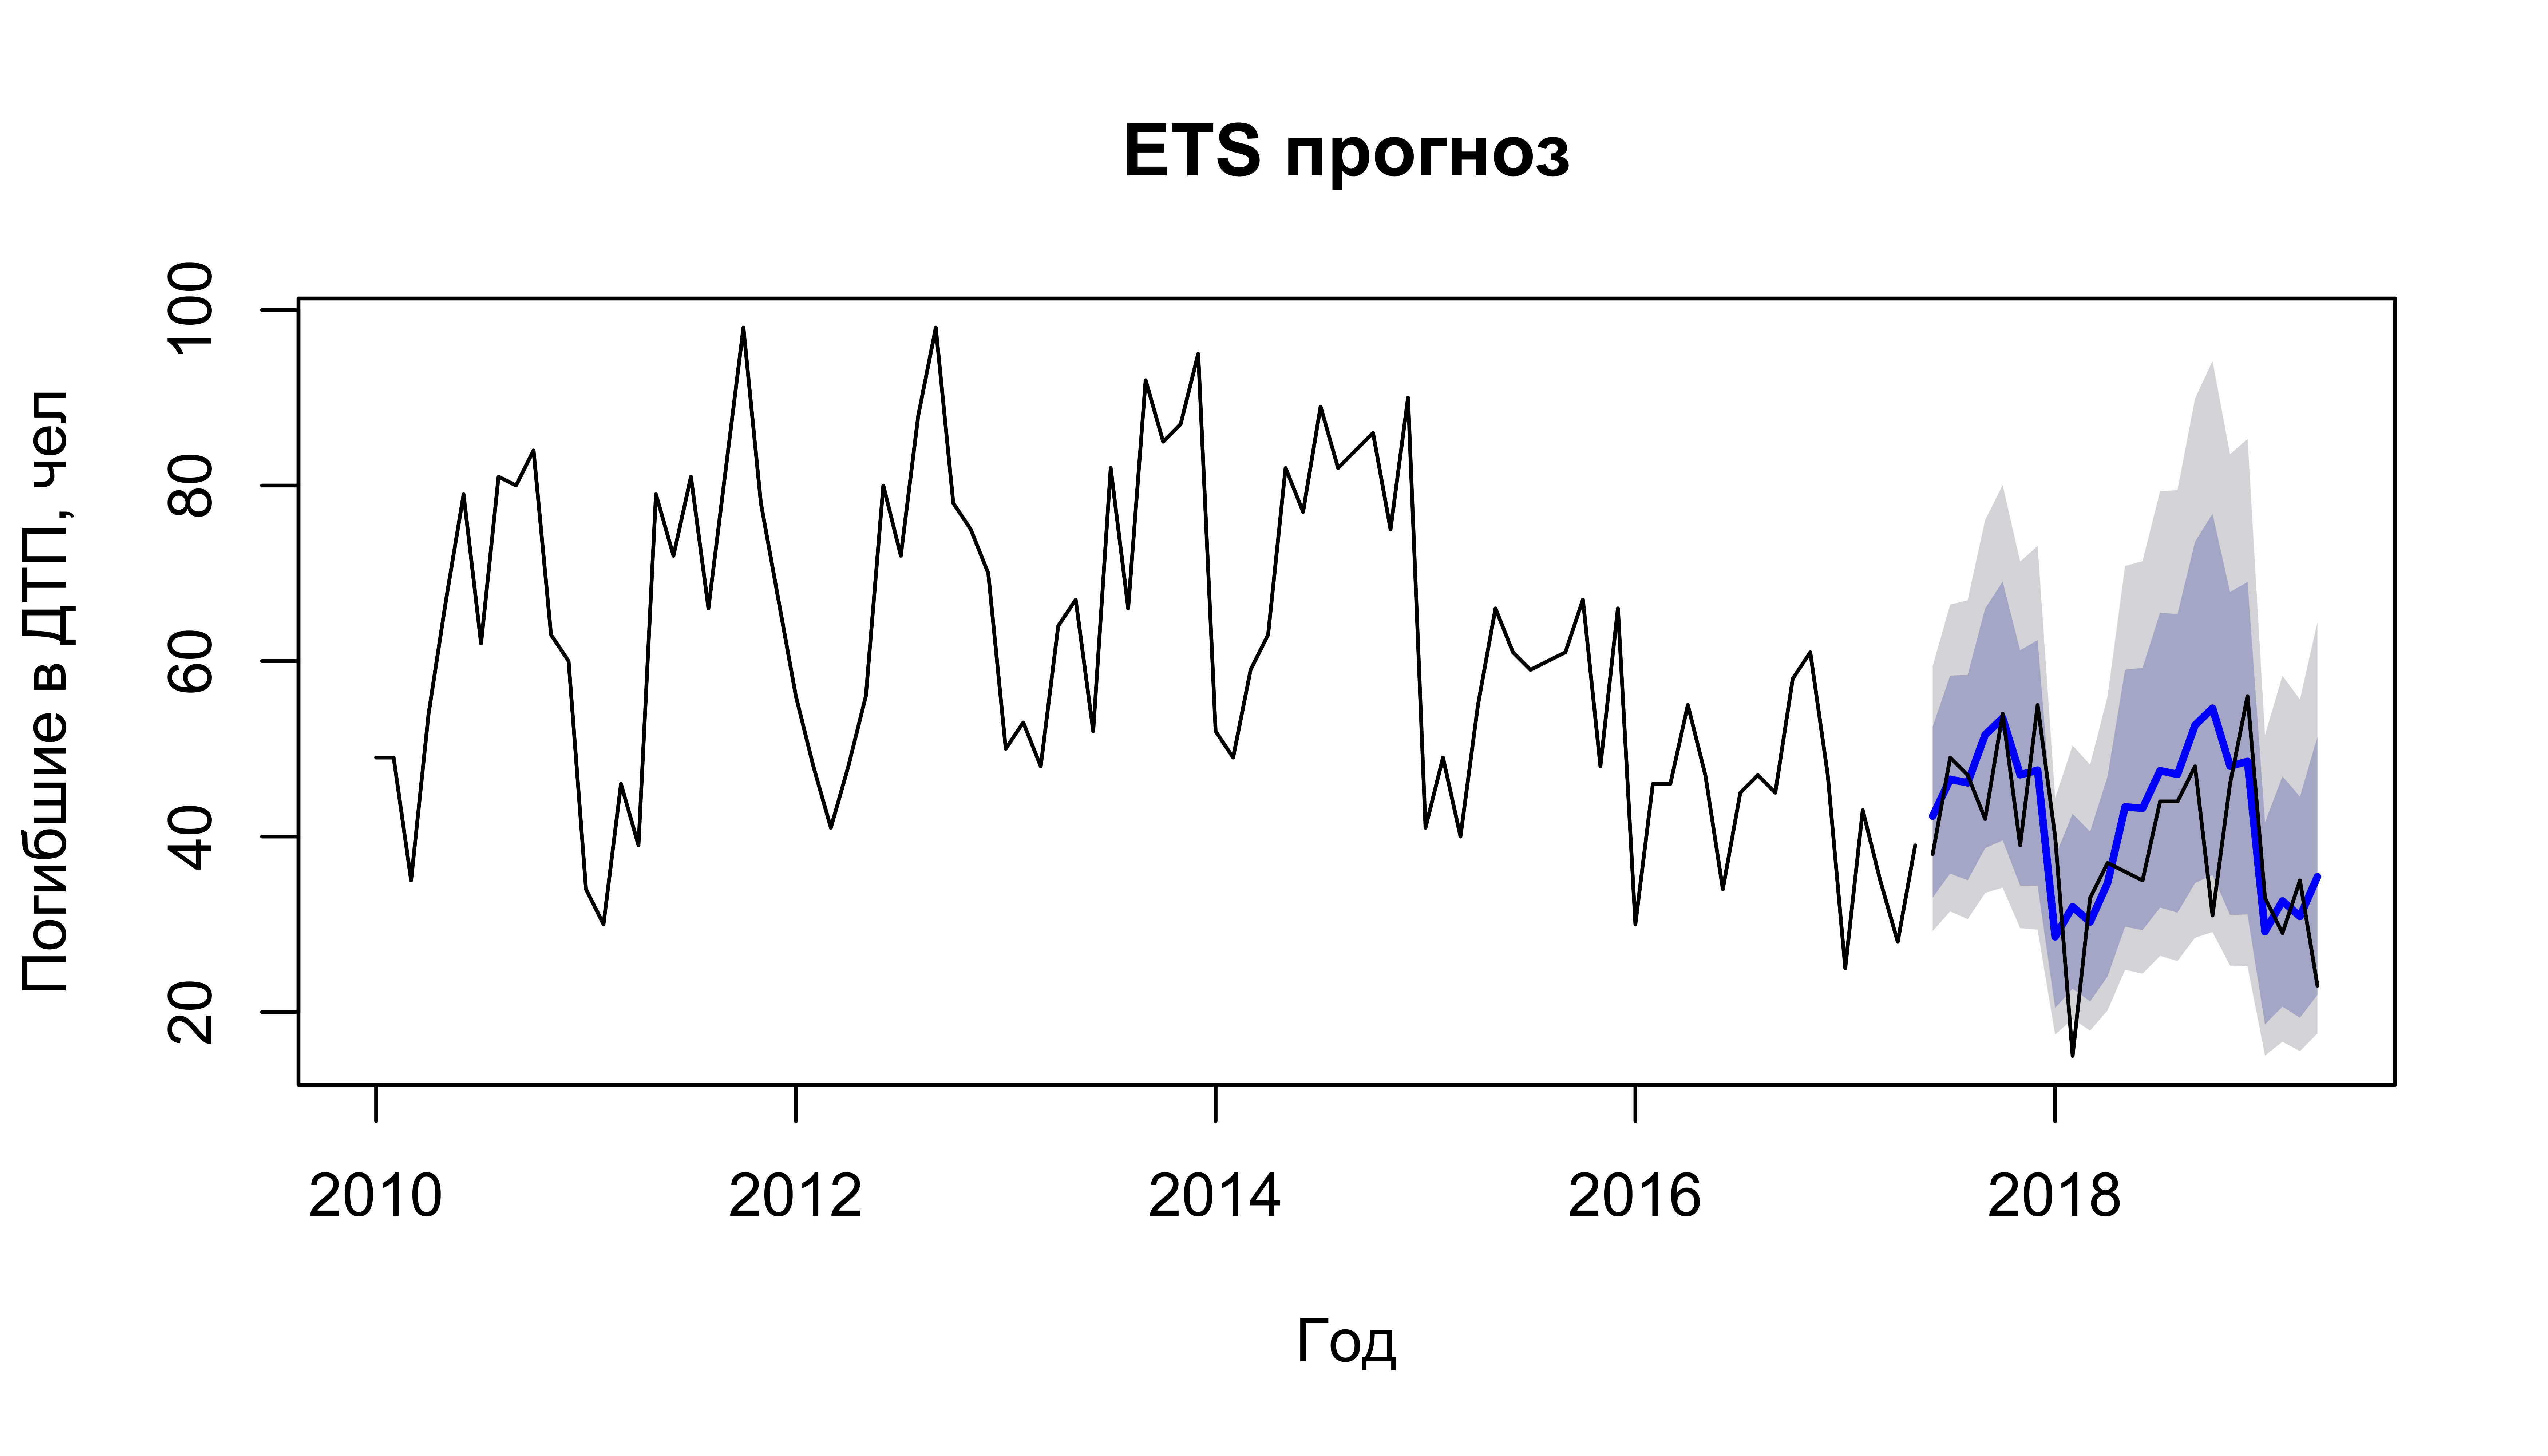
\includegraphics[width=\maxwidth]{figure/unnamed-chunk-18-1} 

}



\end{knitrout}
\end{figure}
\end{minipage}

\begin{minipage}[t]{0.5\textwidth}
\begin{figure}[H]
\begin{knitrout}
\definecolor{shadecolor}{rgb}{0.969, 0.969, 0.969}\color{fgcolor}

{\centering 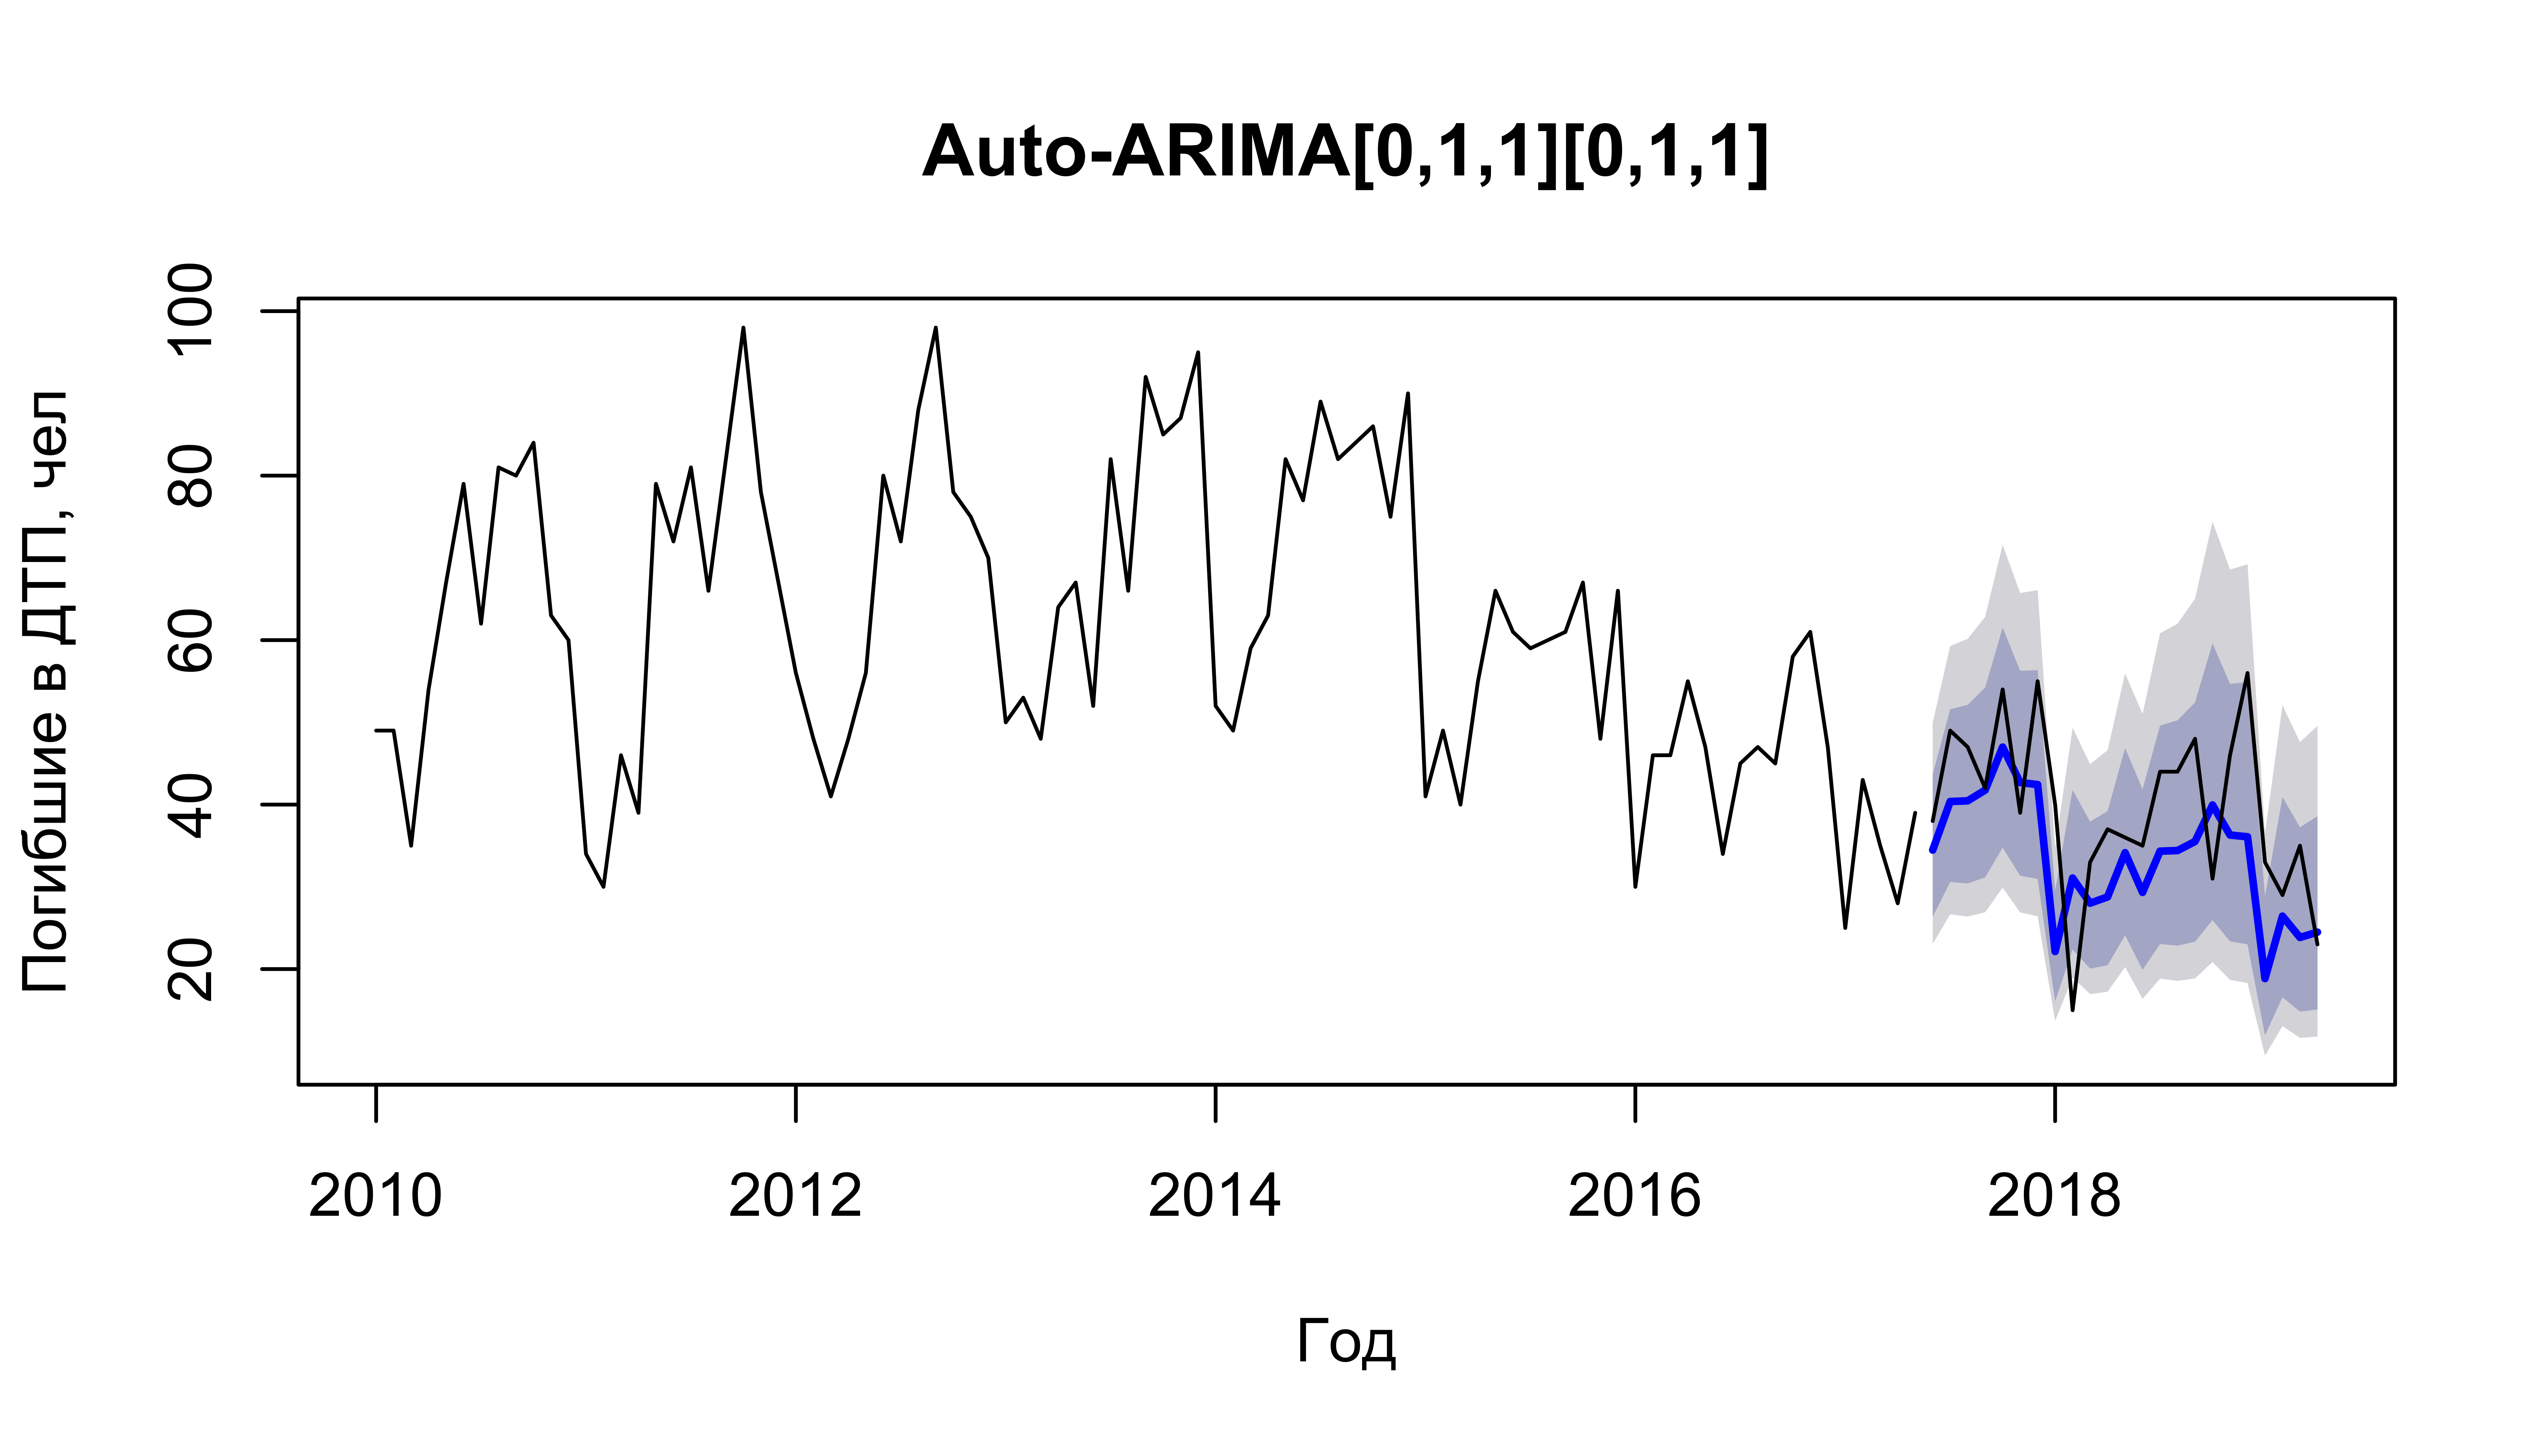
\includegraphics[width=\maxwidth]{figure/unnamed-chunk-19-1} 

}



\end{knitrout}
\end{figure}
\end{minipage}

\begin{minipage}[t]{0.5\textwidth}
\begin{figure}[H]
\begin{knitrout}
\definecolor{shadecolor}{rgb}{0.969, 0.969, 0.969}\color{fgcolor}

{\centering 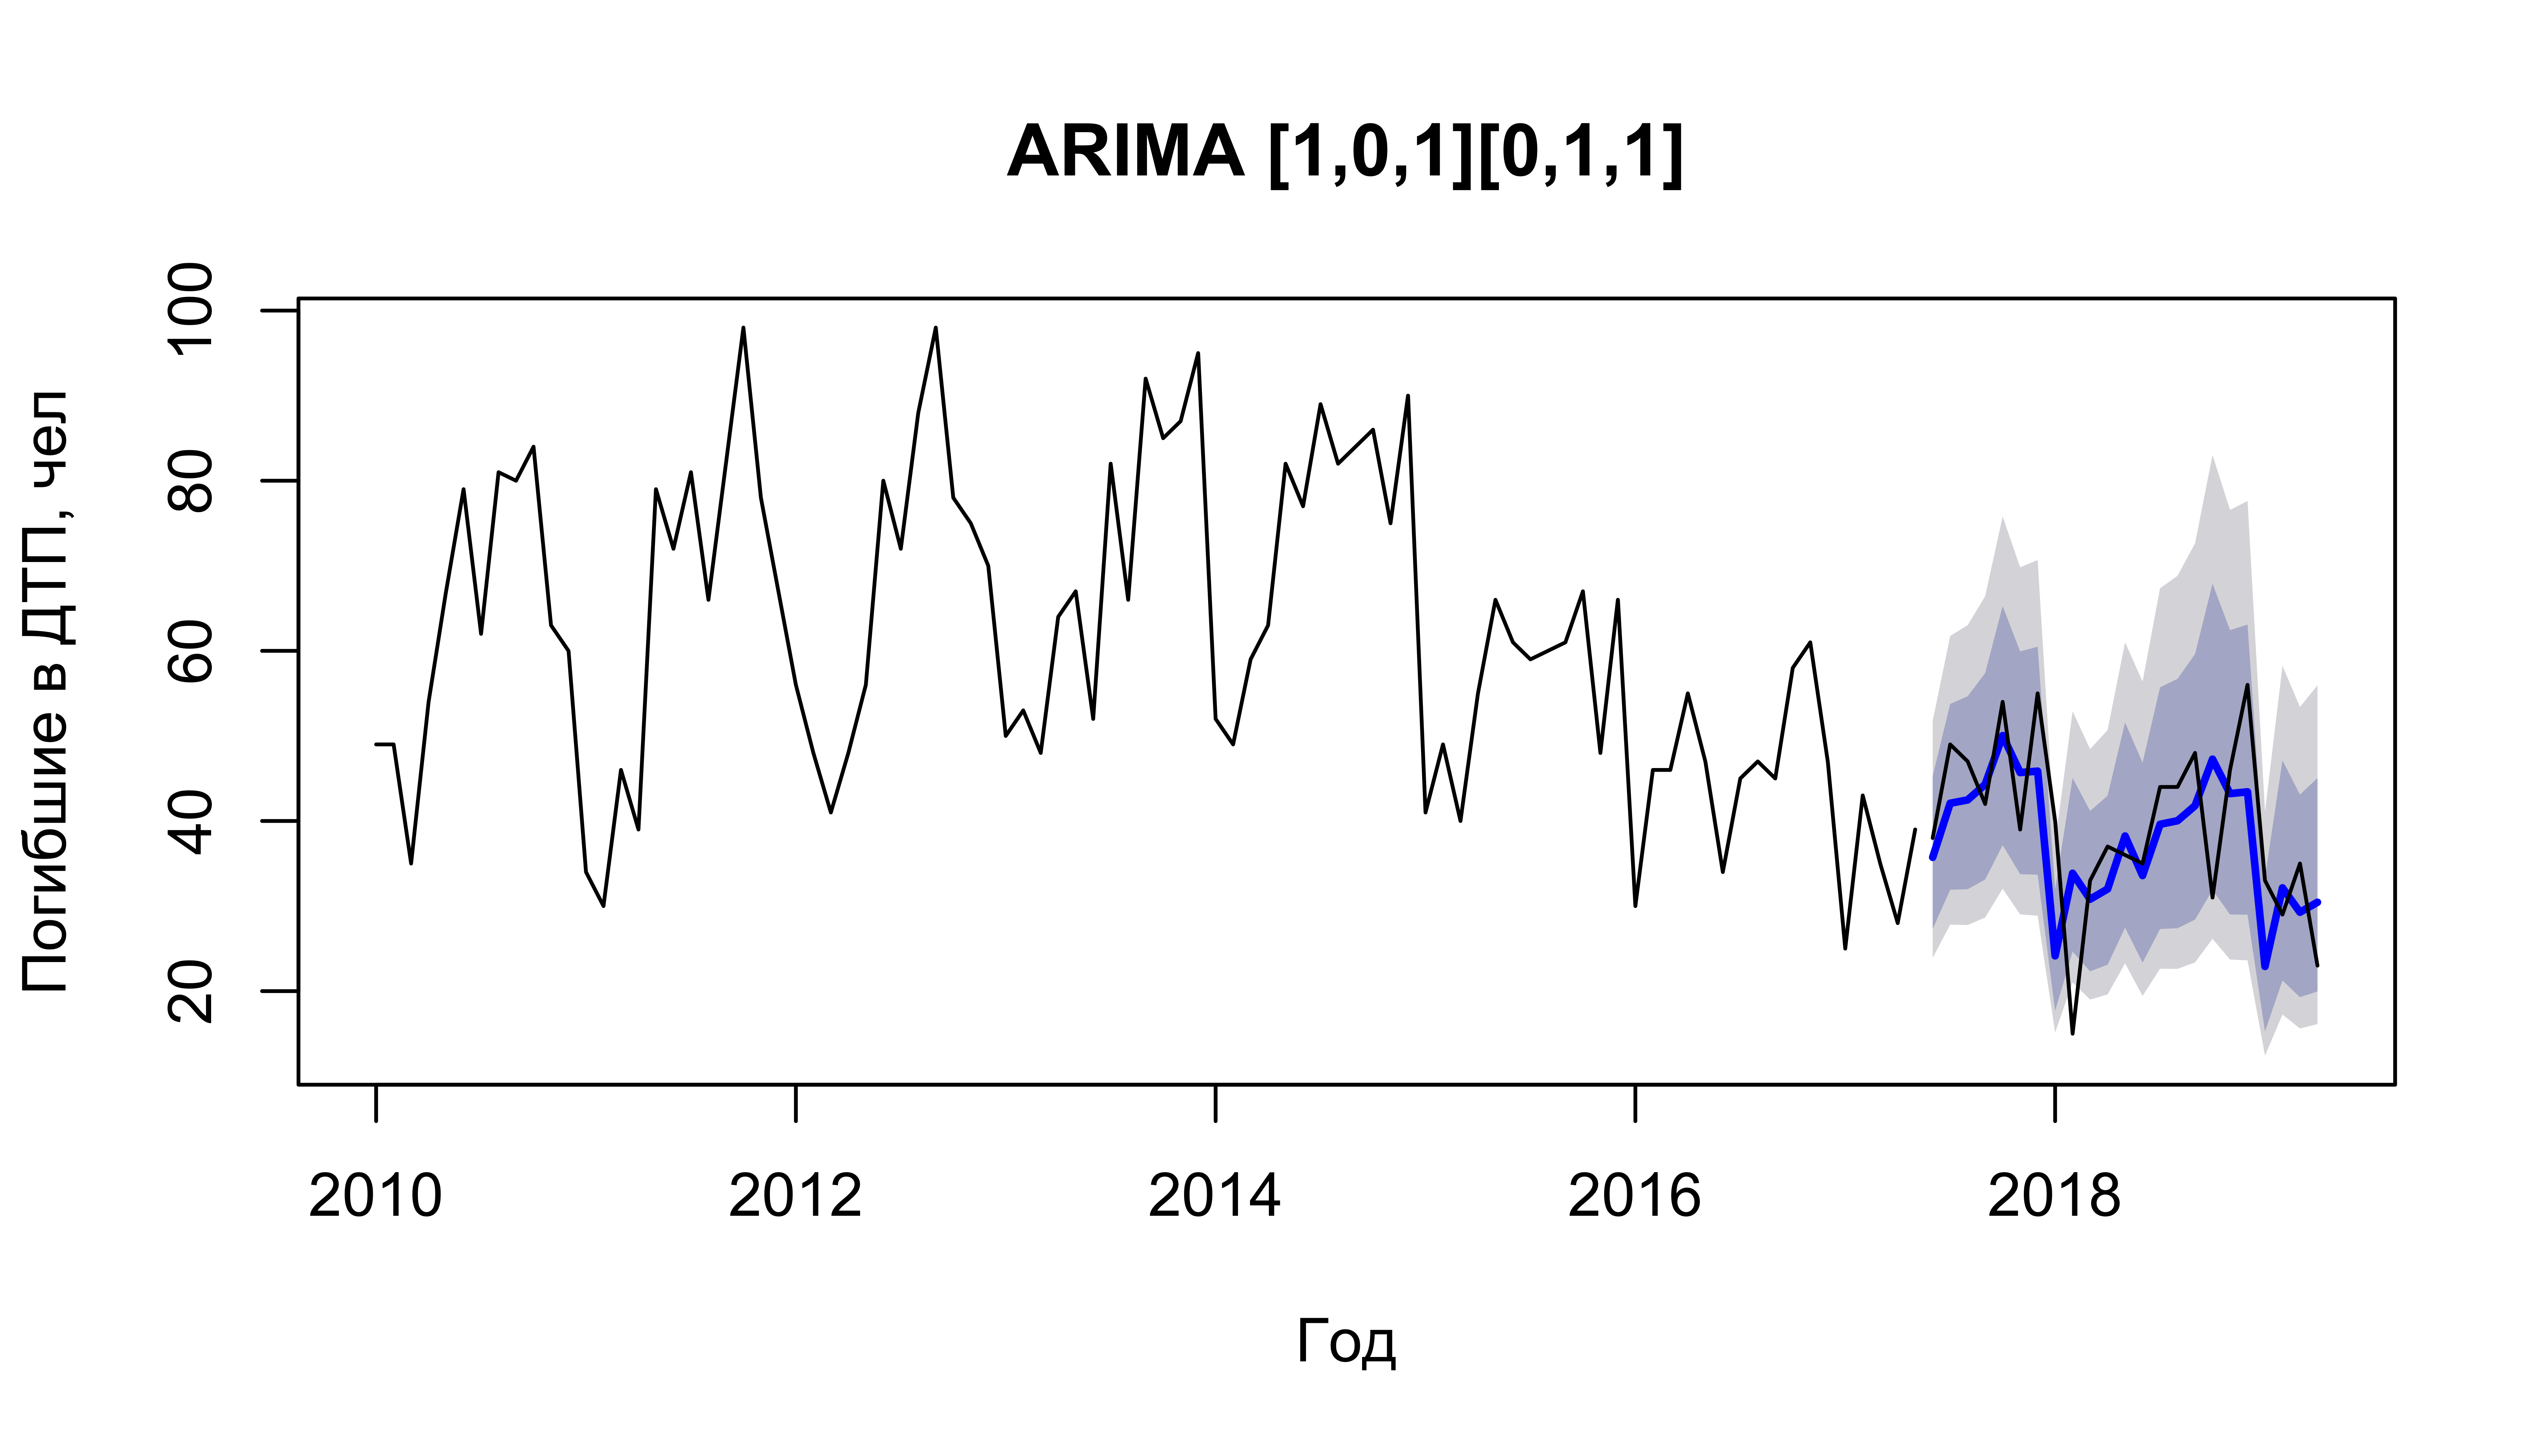
\includegraphics[width=\maxwidth]{figure/unnamed-chunk-20-1} 

}



\end{knitrout}
\end{figure}
\end{minipage}

Таким образом, из имеющихся моделей более хорошей для описания существующих данных оказывается модель с дамми переменной: ARIMA[1,0,1][0,1,1][12], в то время как для прогнозирования больше подходит та же модель, но без дамми-переменной. 

Тесты:
\begin{enumerate}
\item Проверю остатки моделей через тест Льюнга-Бокса на их некоррелированность между собой. Р-значение велико. Это значит, что гипотеза о равенстве нулю автокорреляционной функции остатков модели не отвергается. 
\begin{figure}[H]
\begin{knitrout}
\definecolor{shadecolor}{rgb}{0.914, 0.988, 0.89}\color{fgcolor}\begin{kframe}
\begin{verbatim}
## 
## 	Ljung-Box test
## 
## data:  Residuals from Regression with ARIMA(1,0,1)(0,1,1)[12] errors
## Q* = 17.828, df = 18, p-value = 0.467
## 
## Model df: 4.   Total lags used: 22
\end{verbatim}
\end{kframe}
\end{knitrout}
\end{figure}
\begin{figure}[H]
\begin{knitrout}
\definecolor{shadecolor}{rgb}{0.914, 0.988, 0.89}\color{fgcolor}\begin{kframe}
\begin{verbatim}
## 
## 	Ljung-Box test
## 
## data:  Residuals from ARIMA(1,0,1)(0,1,1)[12]
## Q* = 19.475, df = 19, p-value = 0.4267
## 
## Model df: 3.   Total lags used: 22
\end{verbatim}
\end{kframe}
\end{knitrout}
\end{figure}

\item Далее - тест Харке-Берра. По его результатам обе модели имеют ненормальные остатки. Это очень грустно.
\begin{knitrout}
\definecolor{shadecolor}{rgb}{0.988, 0.89, 0.89}\color{fgcolor}\begin{kframe}
\begin{verbatim}
## 
## 	Jarque Bera Test
## 
## data:  resid(auto(dtp_ts, 1, 112))
## X-squared = 39.984, df = 2, p-value = 2.077e-09
\end{verbatim}
\end{kframe}
\end{knitrout}


\begin{knitrout}
\definecolor{shadecolor}{rgb}{0.988, 0.89, 0.89}\color{fgcolor}\begin{kframe}
\begin{verbatim}
## 
## 	Jarque Bera Test
## 
## data:  resid(bez_d(dtp_ts))
## X-squared = 31.565, df = 2, p-value = 1.399e-07
\end{verbatim}
\end{kframe}
\end{knitrout}

\item ARCH-тест для проверки гомоскедостичности остатков:

\begin{knitrout}
\definecolor{shadecolor}{rgb}{0.914, 0.988, 0.89}\color{fgcolor}\begin{kframe}
\begin{verbatim}
## ARCH heteroscedasticity test for residuals 
## alternative: heteroscedastic 
## 
## Portmanteau-Q test: 
##      order    PQ p.value
## [1,]     4  2.94   0.568
## [2,]     8  6.13   0.632
## [3,]    12  9.05   0.698
## [4,]    16 10.64   0.831
## [5,]    20 16.44   0.689
## [6,]    24 16.73   0.860
## Lagrange-Multiplier test: 
##      order    LM  p.value
## [1,]     4 69.15 6.44e-15
## [2,]     8 28.37 1.88e-04
## [3,]    12 12.69 3.14e-01
## [4,]    16  8.77 8.89e-01
## [5,]    20  4.58 1.00e+00
## [6,]    24  1.86 1.00e+00
\end{verbatim}
\end{kframe}
\end{knitrout}

\begin{knitrout}
\definecolor{shadecolor}{rgb}{0.914, 0.988, 0.89}\color{fgcolor}\begin{kframe}
\begin{verbatim}
## ARCH heteroscedasticity test for residuals 
## alternative: heteroscedastic 
## 
## Portmanteau-Q test: 
##      order    PQ p.value
## [1,]     4  2.94   0.568
## [2,]     8  6.13   0.632
## [3,]    12  9.05   0.698
## [4,]    16 10.64   0.831
## [5,]    20 16.44   0.689
## [6,]    24 16.73   0.860
## Lagrange-Multiplier test: 
##      order    LM  p.value
## [1,]     4 69.15 6.44e-15
## [2,]     8 28.37 1.88e-04
## [3,]    12 12.69 3.14e-01
## [4,]    16  8.77 8.89e-01
## [5,]    20  4.58 1.00e+00
## [6,]    24  1.86 1.00e+00
\end{verbatim}
\end{kframe}
\end{knitrout}
\end{enumerate}

Значит, с точки зрения качества остатков эти модели примерно одинаковы. Для прогноза я возьму модель  ARIMA[1,0,1][0,1,1][12] без дамми-переменной.

\subsection{Прогнозирование}

Теперь сделаем прогноз на два года  вперед.
числовой прогноз:



% latex table generated in R 3.5.3 by xtable 1.8-4 package
% Sun Jun  2 15:55:35 2019
\begin{table}[ht]
\centering
\begin{tabular}{rrrrrr}
  \hline
 & Point Forecast & Lo 80 & Hi 80 & Lo 95 & Hi 95 \\ 
  \hline
May 2019 & 37.81 & 28.18 & 48.80 & 24.39 & 56.47 \\ 
  Jun 2019 & 35.55 & 26.39 & 46.07 & 22.79 & 53.43 \\ 
  Jul 2019 & 42.26 & 31.22 & 55.02 & 26.89 & 63.97 \\ 
  Aug 2019 & 42.06 & 30.95 & 54.99 & 26.60 & 64.07 \\ 
  Sep 2019 & 43.90 & 32.17 & 57.62 & 27.59 & 67.28 \\ 
  Oct 2019 & 43.34 & 31.65 & 57.11 & 27.09 & 66.81 \\ 
  Nov 2019 & 41.93 & 30.51 & 55.44 & 26.06 & 64.98 \\ 
  Dec 2019 & 47.17 & 34.19 & 62.62 & 29.15 & 73.56 \\ 
  Jan 2020 & 27.89 & 20.19 & 37.09 & 17.20 & 43.60 \\ 
  Feb 2020 & 25.76 & 18.59 & 34.35 & 15.82 & 40.45 \\ 
  Mar 2020 & 29.85 & 21.46 & 39.95 & 18.22 & 47.13 \\ 
  Apr 2020 & 29.23 & 20.96 & 39.25 & 17.76 & 46.38 \\ 
  May 2020 & 36.40 & 25.61 & 49.80 & 21.50 & 59.43 \\ 
  Jun 2020 & 34.24 & 23.99 & 47.04 & 20.09 & 56.27 \\ 
  Jul 2020 & 40.71 & 28.38 & 56.21 & 23.70 & 67.42 \\ 
  Aug 2020 & 40.54 & 28.14 & 56.21 & 23.46 & 67.57 \\ 
  Sep 2020 & 42.32 & 29.26 & 58.93 & 24.33 & 71.00 \\ 
  Oct 2020 & 41.80 & 28.78 & 58.43 & 23.89 & 70.54 \\ 
  Nov 2020 & 40.45 & 27.75 & 56.75 & 22.99 & 68.65 \\ 
  Dec 2020 & 45.53 & 31.10 & 64.14 & 25.71 & 77.76 \\ 
  Jan 2021 & 26.94 & 18.39 & 38.00 & 15.19 & 46.10 \\ 
  Feb 2021 & 24.88 & 16.93 & 35.22 & 13.96 & 42.80 \\ 
  Mar 2021 & 28.84 & 19.55 & 40.98 & 16.09 & 49.91 \\ 
  Apr 2021 & 28.26 & 19.09 & 40.28 & 15.68 & 49.13 \\ 
   \hline
\end{tabular}
\caption{Числовой прогноз на 24 месяца} 
\end{table}



\begin{figure}[H]
\begin{knitrout}
\definecolor{shadecolor}{rgb}{0.969, 0.969, 0.969}\color{fgcolor}

{\centering 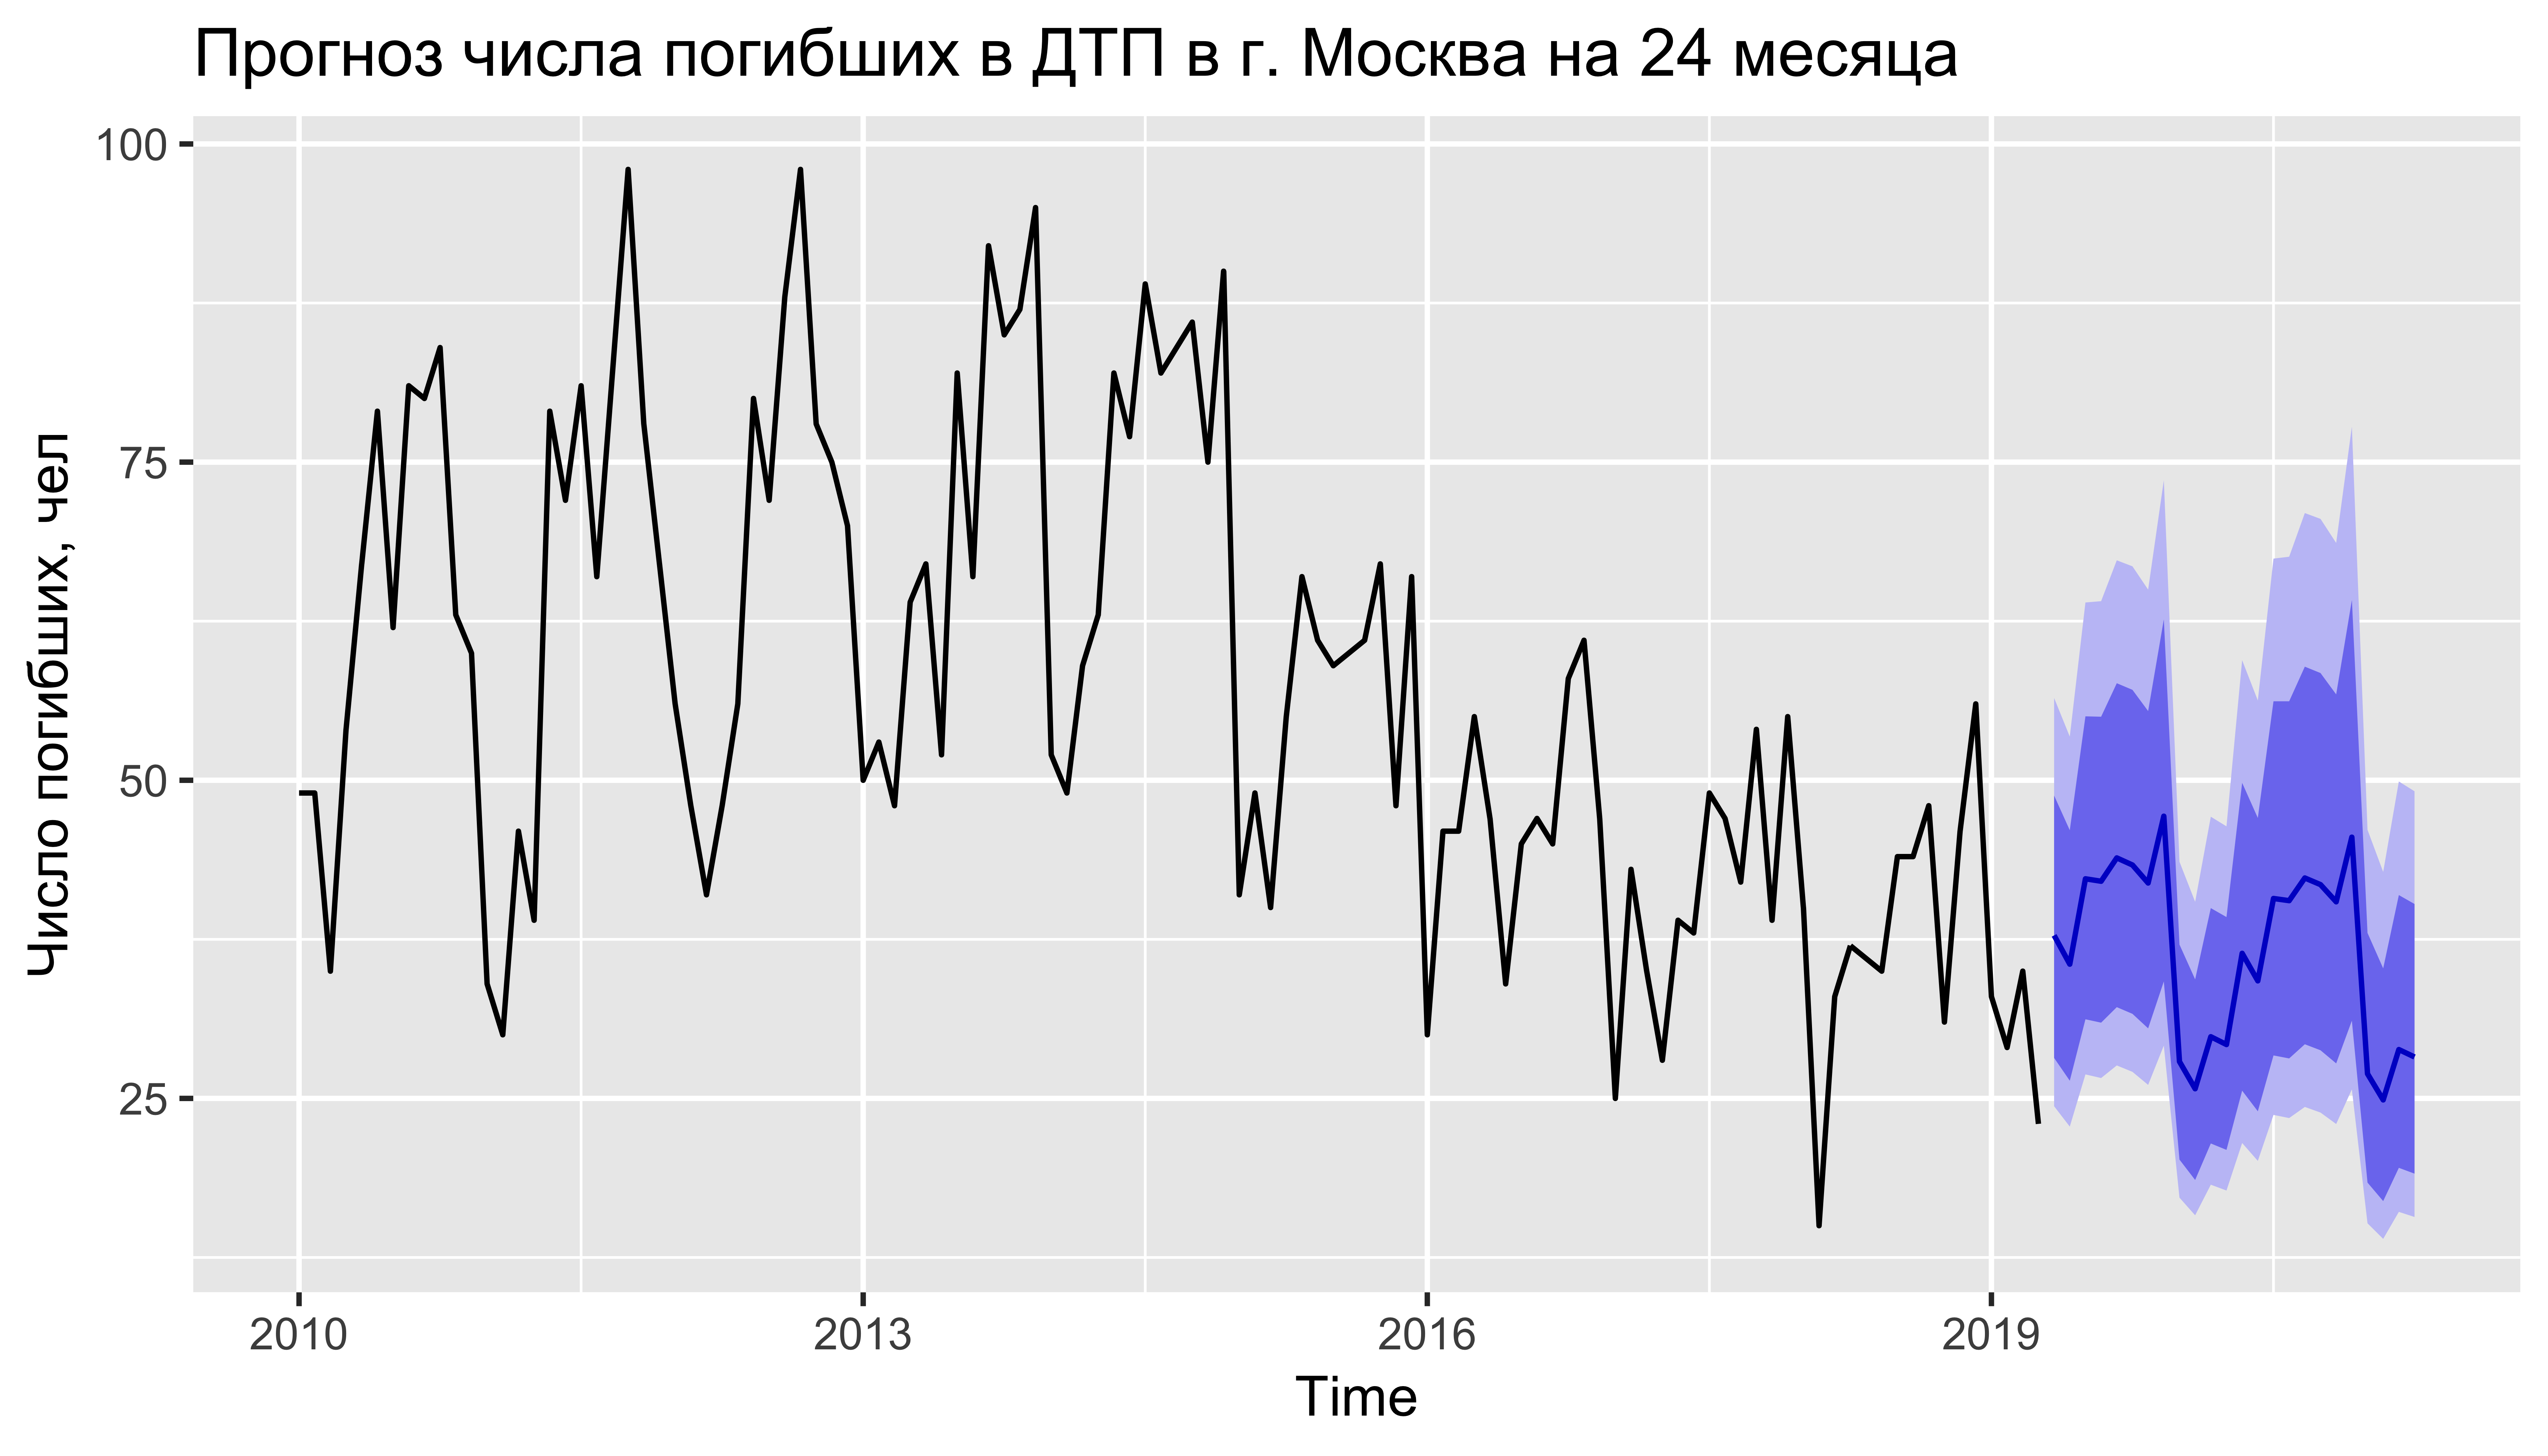
\includegraphics[width=\maxwidth]{figure/unnamed-chunk-29-1} 

}



\end{knitrout}
\end{figure}



% latex table generated in R 3.5.3 by xtable 1.8-4 package
% Sun Jun  2 15:55:37 2019
\begin{table}[ht]
\centering
\begin{tabular}{rrrrrr}
  \hline
 & Point Forecast & Lo 80 & Hi 80 & Lo 95 & Hi 95 \\ 
  \hline
May 2019 & 40.09 & 30.42 & 50.81 & 26.57 & 58.23 \\ 
  Jun 2019 & 40.06 & 30.17 & 51.05 & 26.26 & 58.72 \\ 
  Jul 2019 & 44.50 & 33.24 & 57.03 & 28.84 & 65.82 \\ 
  Aug 2019 & 44.26 & 32.83 & 57.02 & 28.38 & 66.04 \\ 
  Sep 2019 & 47.58 & 35.02 & 61.62 & 30.18 & 71.61 \\ 
  Oct 2019 & 49.22 & 35.97 & 64.07 & 30.90 & 74.70 \\ 
  Nov 2019 & 44.31 & 32.18 & 57.95 & 27.56 & 67.76 \\ 
  Dec 2019 & 47.39 & 34.17 & 62.29 & 29.17 & 73.08 \\ 
  Jan 2020 & 28.48 & 20.44 & 37.55 & 17.42 & 44.13 \\ 
  Feb 2020 & 27.67 & 19.74 & 36.64 & 16.77 & 43.20 \\ 
  Mar 2020 & 28.73 & 20.36 & 38.22 & 17.25 & 45.20 \\ 
  Apr 2020 & 32.01 & 22.53 & 42.78 & 19.02 & 50.74 \\ 
  May 2020 & 40.59 & 28.36 & 54.53 & 23.87 & 64.89 \\ 
  Jun 2020 & 40.56 & 28.16 & 54.72 & 23.64 & 65.30 \\ 
  Jul 2020 & 45.05 & 31.07 & 61.05 & 26.01 & 73.07 \\ 
  Aug 2020 & 44.81 & 30.72 & 60.97 & 25.65 & 73.17 \\ 
  Sep 2020 & 48.17 & 32.81 & 65.81 & 27.32 & 79.20 \\ 
  Oct 2020 & 49.83 & 33.74 & 68.35 & 28.01 & 82.49 \\ 
  Nov 2020 & 44.86 & 30.21 & 61.75 & 25.03 & 74.69 \\ 
  Dec 2020 & 47.98 & 32.12 & 66.31 & 26.54 & 80.43 \\ 
  Jan 2021 & 28.83 & 19.24 & 39.92 & 15.88 & 48.48 \\ 
  Feb 2021 & 28.01 & 18.59 & 38.92 & 15.30 & 47.38 \\ 
  Mar 2021 & 29.08 & 19.19 & 40.57 & 15.76 & 49.51 \\ 
  Apr 2021 & 32.40 & 21.25 & 45.37 & 17.41 & 55.52 \\ 
   \hline
\end{tabular}
\caption{ETS Числовой прогноз на 24 месяца} 
\end{table}



\begin{figure}[H]
\begin{knitrout}
\definecolor{shadecolor}{rgb}{0.969, 0.969, 0.969}\color{fgcolor}

{\centering 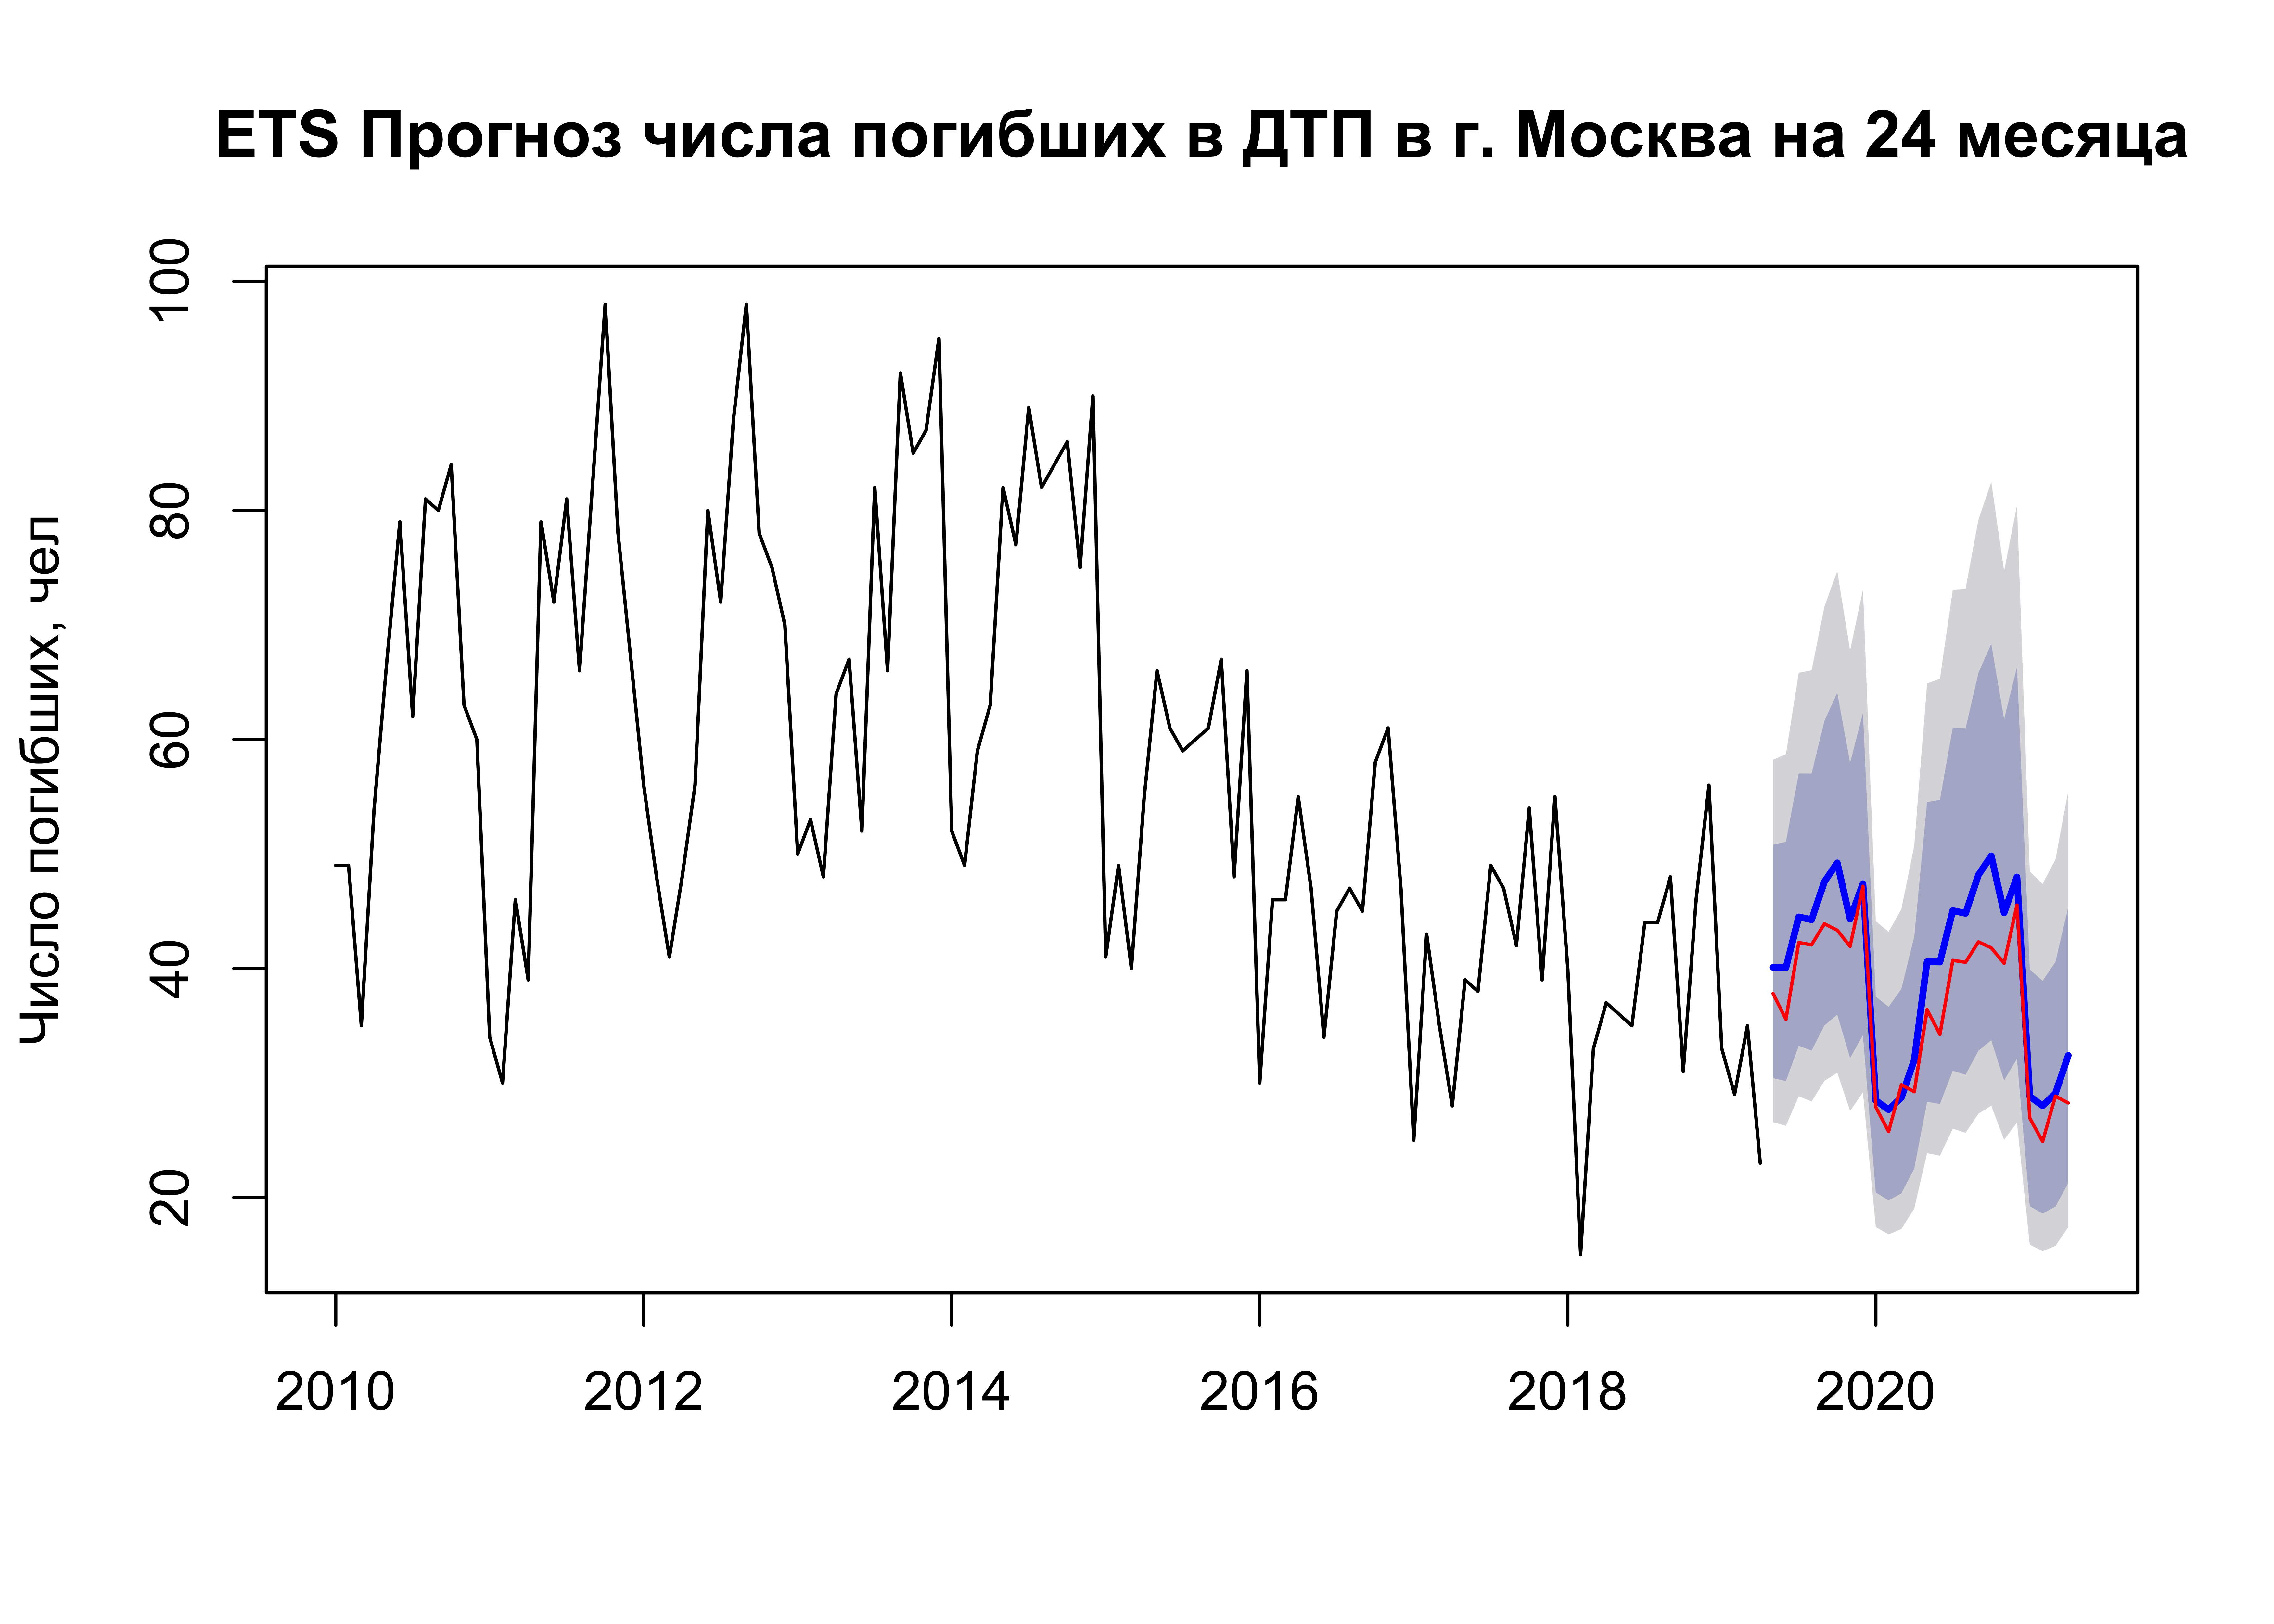
\includegraphics[width=\maxwidth]{figure/unnamed-chunk-32-1} 

}



\end{knitrout}
\end{figure}

\end{document}
